\pdfminorversion=6 % this is needed to be able to include pdf 1.6. 
                    % For some reasons some old HPSG proceedings have pdf 1.6
\documentclass[11pt,a4paper,fleqn]{article}
\usepackage{times}
\thispagestyle{empty}



\usepackage[T1]{fontenc}   % Silbentrennung

\usepackage[utf8x]{inputenc}
                                                                                                                             
\hyphenation{Acad-e-my}

\usepackage[bookmarks=true,bookmarksopen=true,%
breaklinks=true,%
draft=false,plainpages=false,hyperfootnotes=false,%
pdfauthor={Stefan Müller (Editor)},%
pdftitle={Proceedings of the 17th International Conference on Head-Driven Phrase Structure Grammar},%
pdfkeywords={HPSG}%,
pdftex=true%
%ps2pdf=true  %ohne diesen Treiber geht der Zeilenumbruch in URLs
]{hyperref}% for pdf files
\hypersetup{colorlinks=false, pdfborder={0 0 0}}

\usepackage{pdfpages}
\pdfinclusioncopyfonts=1

\newcommand\formatauthor[2]{\begin{tabular}[t]{@{}c@{}}
  {\LARGE#1\strut}\\
  {\small#2\strut}\\
  \rule{\dimexpr0.5\linewidth-1em}{0pt}
  \end{tabular}\xhfill\ignorespaces}
\newcommand\xhfill{\hspace{1em plus 1fill}}

\begin{document}

\begin{center}
{\Large
                {\bfseries Proceedings of the 17th International Conference on\par Head-Driven Phrase Structure Grammar\par}

                \vspace{8ex}

                     Universit{\'e} Paris Diderot, Paris 7, France\\[\baselineskip]

                        Stefan M{\"u}ller (Editor)\\[\baselineskip]

                                2010\\[\baselineskip]

                          CSLI Publications\\[\baselineskip]

              http://csli-publications.stanford.edu/HPSG/2010 \\[4\baselineskip]

The papers are published under a \href{http://creativecommons.org/licenses/by/4.0/}{CC-BY license}:\\[3pt]
\href{http://creativecommons.org/licenses/by/4.0/}{http://creativecommons.org/licenses/by/4.0/}
}
\end{center}
\newpage
\tableofcontents

\newpage

\section{Editor's Note}
%% -*- coding:utf-8 -*-
The 17th International Conference on Head-Driven Phrase Structure Grammar (2010) was held at Université Paris Diderot, Paris 7.

The conference featured 2 invited talks and 19 papers, and 5 posters selected by the program committee (Doug Arnold,
Emily M. Bender, Philippe Blache, Olivier Bonami (chair), Bob Borsley, Gosse Bouma, Rui Chaves, Ann
Copestake,
Berthold Crysmann, Kordula De Kuthy, Dan Flickinger, Daniele Godard, Anke Holler, Jean-Pierre
Koenig, Valia Kordoni, Anna Kupsc, Bob Levine, Rob Malouf, Nurit Melnik, Philip Miller, Stefan
Müller, Gerald Penn, Frank Richter, Ivan Sag, Manfred Sailer, Jesse Tseng, Frank Van Eynde, Gert
Webelhuth, Shuichi Yatabe, Eun-Jung Yoo).

A workshop about \emph{Morphology and Formal Grammar}
was attached to the conference. It featured one invited talk and 10 papers and three posters, selected by the program
committee of this workshop (Farrell Ackerman,
Emily Bender,
James Blevins,
Olivier Bonami (chair),
Dunstan Brown,
Gilles Boyé,
Berthold Crysmann,
Bernard Fradin,
Rob Malouf,
Stefan Müller,
Louisa Sadler,
Pollet Samvelian,
Andrew Spencer,
Jesse Tseng,
Gert Webelhuth).


In total there were 29  submissions to the conference and 24 submissions to the workshop.
We want to thank the respective program committees for putting this nice program together.



Thanks go to Anne Abeillé (chair), Gabriela Bilbîie, Olivier Bonami, Marianne Desmets, Danièle Godard,
Fabiola Henri,
Frédéric Laurens,
Philip Miller,
François Mouret,
Clément Plancq,
Jana Strnadová,
Delphine Tribout,
Géraldine Walter,
Grégoire Winterstein, who were in charge of local arrangements.


As in the past years the contributions to the conference proceedings are based on the five page abstract
that was reviewed by the respective program committees, but there is no additional reviewing of the
longer contribution to the proceedings.
To ensure easy access and fast publication we have chosen an electronic format.


The proceedings include all the papers except those by Farrell Ackerman and Rob Malouf, Dan Flickinger, Jean-Pierre Koenig and Karin
Michelson, Robert Levine, Jakob Maché, Nurit Melnik, and Gregory Stump.


\newpage
\part{Contributions to the Main Conference}
\thispagestyle{empty}
\newpage
        \setcounter{page}{6}
        \phantomsection
        \addcontentsline{toc}{section}{Katya Alahverdzhieva, Alex Lascarides: Analysing Speech and Co-Speech Gesture in Constraint-based Grammars}
\thispagestyle{empty}

\begin{center}
  {\huge\bfseries Analysing Speech and Co-Speech Gesture in Constraint-based Grammars\par}

  \bigskip

~\\
\begingroup
\setlength{\leftskip}{0pt plus 1fill}
\setlength{\rightskip}{0pt plus 1fill}
\setlength{\parindent}{0pt}
\setlength{\parfillskip}{0pt}
  \formatauthor{Katya Alahverdzhieva}{\begin{tabular}{@{}c@{}}UNiversity of Edinburgh\end{tabular}}
\formatauthor{Alex Lascarides}{\begin{tabular}{@{}c@{}}UNiversity of Edinburgh\end{tabular}}

\par\endgroup

  \vspace*{8ex}

  Proceedings of the 17th International Conference on\par Head-Driven Phrase Structure Grammar

  \bigskip

  Universit{\'e} Paris Diderot, Paris 7, France

  \medskip

  Stefan Müller (Editor)

  \medskip

  2010

  \medskip

  CSLI Publications

  \medskip

  pages 6--26

  \medskip

  \url{http://csli-publications.stanford.edu/HPSG/2010}
\end{center}
\vfill

\noindent



\vfill
\noindent
% APA Style
Alahverdzhieva, Katya, \& Lascarides, Alex. 2010. Analysing Speech and Co-Speech Gesture in Constraint-based Grammars. In Müller, Stefan (Ed.), \emph{{Proceedings of the 17th International Conference on Head-Driven Phrase Structure Grammar, Universit{\'e} Paris Diderot, Paris 7, France}}, 6--26. Stanford,
CA: CSLI Publications. \hfill\href{http://creativecommons.org/licenses/by/4.0/}{\includegraphics[height=.75em]{Includes/ccby.eps}}

\newpage
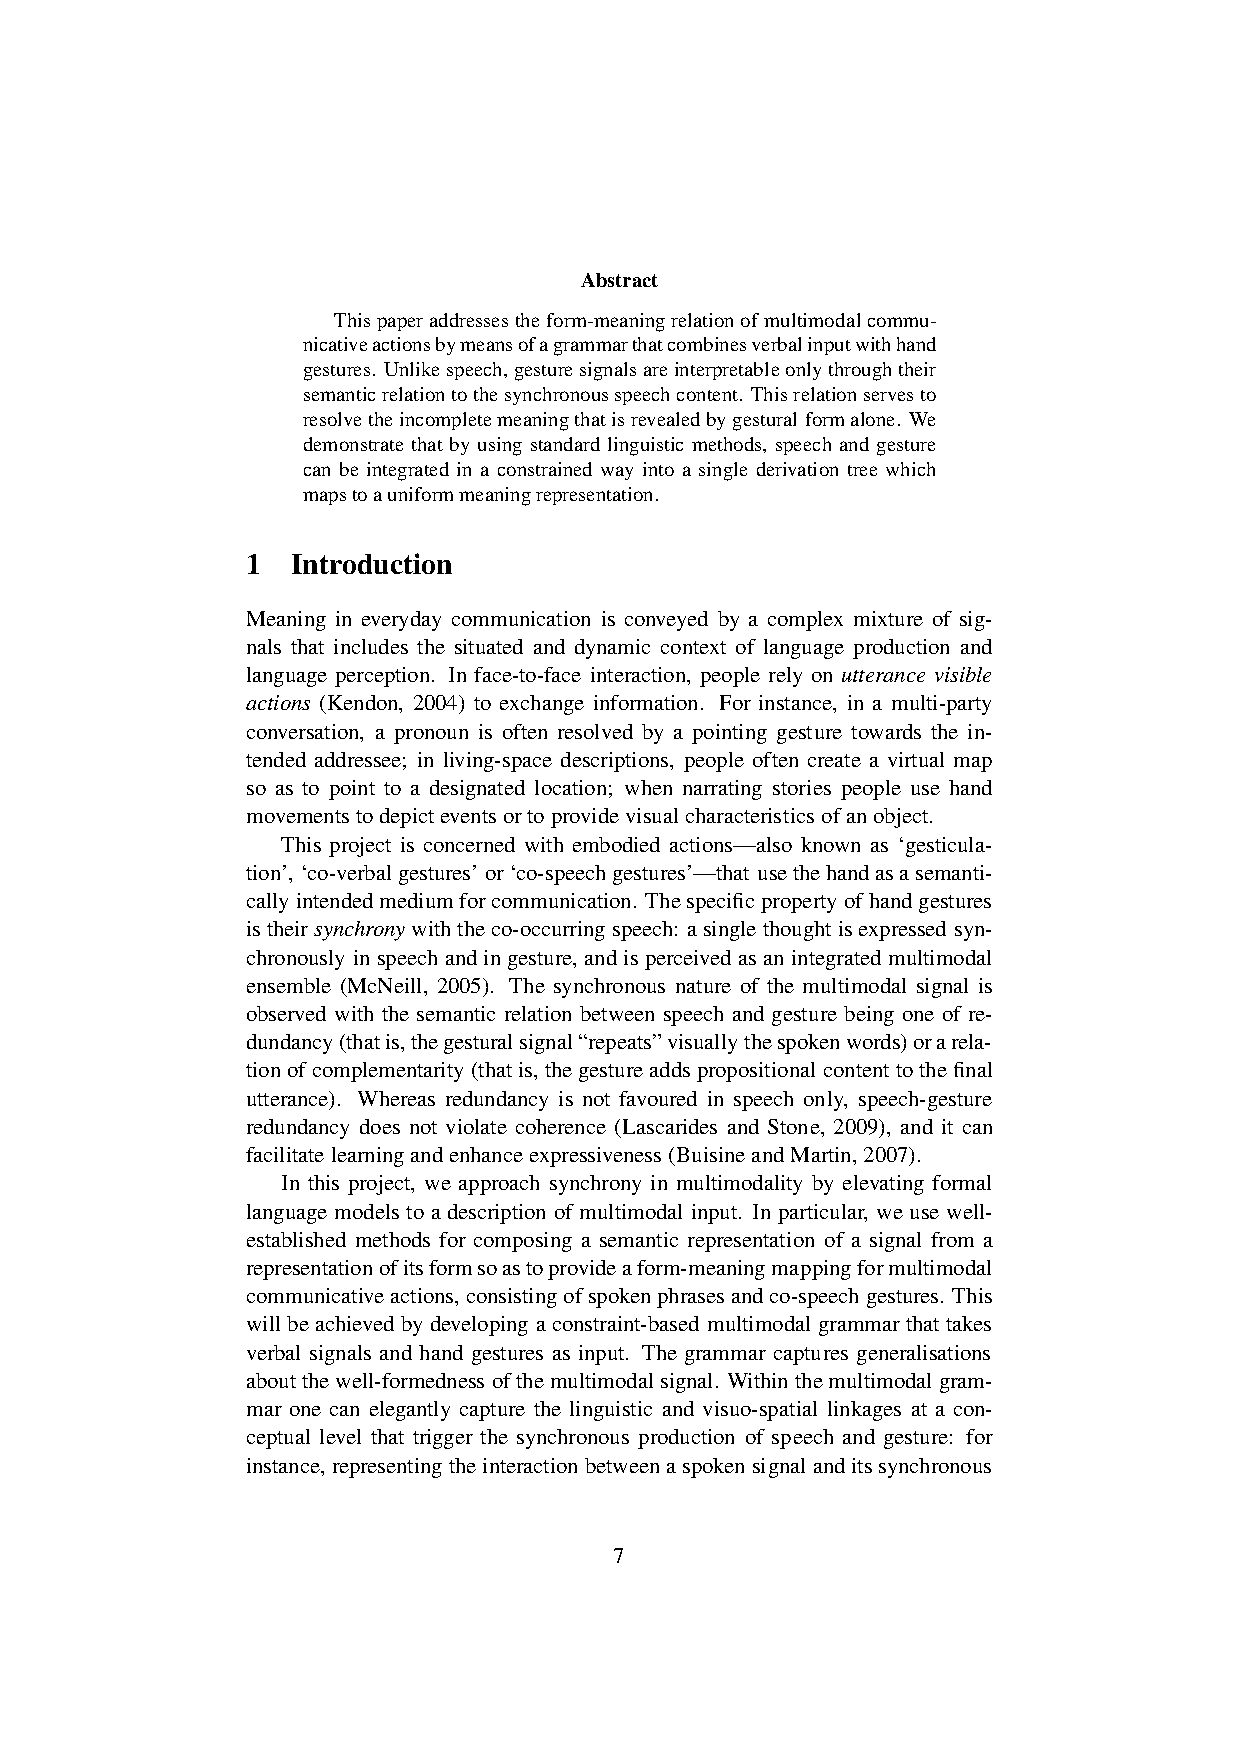
\includepdf[pages=-,pagecommand=\thispagestyle{plain}]{Includes/alahverdzhieva-lascarides.pdf}
        \setcounter{page}{27}
        \phantomsection
        \addcontentsline{toc}{section}{Anke Assmann, Fabian Heck, Johannes Hein, Stefan Keine, Gereon M{\"u}ller: Does Chain Hybridization in Irish Support Movement-Based Approaches to Long-Distance Dependencies?}
\thispagestyle{empty}

\begin{center}
  {\huge\bfseries Does Chain Hybridization in Irish Support Movement-Based Approaches to Long-Distance Dependencies?\par}

  \bigskip

~\\
\begingroup
\setlength{\leftskip}{0pt plus 1fill}
\setlength{\rightskip}{0pt plus 1fill}
\setlength{\parindent}{0pt}
\setlength{\parfillskip}{0pt}
  \formatauthor{Anke Assmann}{\begin{tabular}{@{}c@{}}Universität Leipzig\end{tabular}}
\formatauthor{Fabian Heck}{\begin{tabular}{@{}c@{}}Universität Leipzig\end{tabular}}
\formatauthor{Johannes Hein}{\begin{tabular}{@{}c@{}}Universität Leipzig\end{tabular}}
\formatauthor{Stefan Keine}{\begin{tabular}{@{}c@{}}Universität Leipzig\end{tabular}}
\formatauthor{Gereon Müller}{\begin{tabular}{@{}c@{}}Universität Leipzig\end{tabular}}

\par\endgroup

  \vspace*{8ex}

  Proceedings of the 17th International Conference on\par Head-Driven Phrase Structure Grammar

  \bigskip

  Universit{\'e} Paris Diderot, Paris 7, France

  \medskip

  Stefan Müller (Editor)

  \medskip

  2010

  \medskip

  CSLI Publications

  \medskip

  pages 27--46

  \medskip

  \url{http://csli-publications.stanford.edu/HPSG/2010}
\end{center}
\vfill

\noindent



\vfill
\noindent
% APA Style
Assmann, Anke, Heck, Fabian, Hein, Johannes, Keine, Stefan, \& Müller,  Gereon. 2010. Does Chain Hybridization in Irish Support Movement-Based Approaches to Long-Distance Dependencies? In Müller, Stefan (Ed.), \emph{{Proceedings of the 17th International Conference on Head-Driven Phrase Structure Grammar, Universit{\'e} Paris Diderot, Paris 7, France}}, 27--46. Stanford,
CA: CSLI Publications. \hfill\href{http://creativecommons.org/licenses/by/4.0/}{\includegraphics[height=.75em]{Includes/ccby.eps}}

\newpage
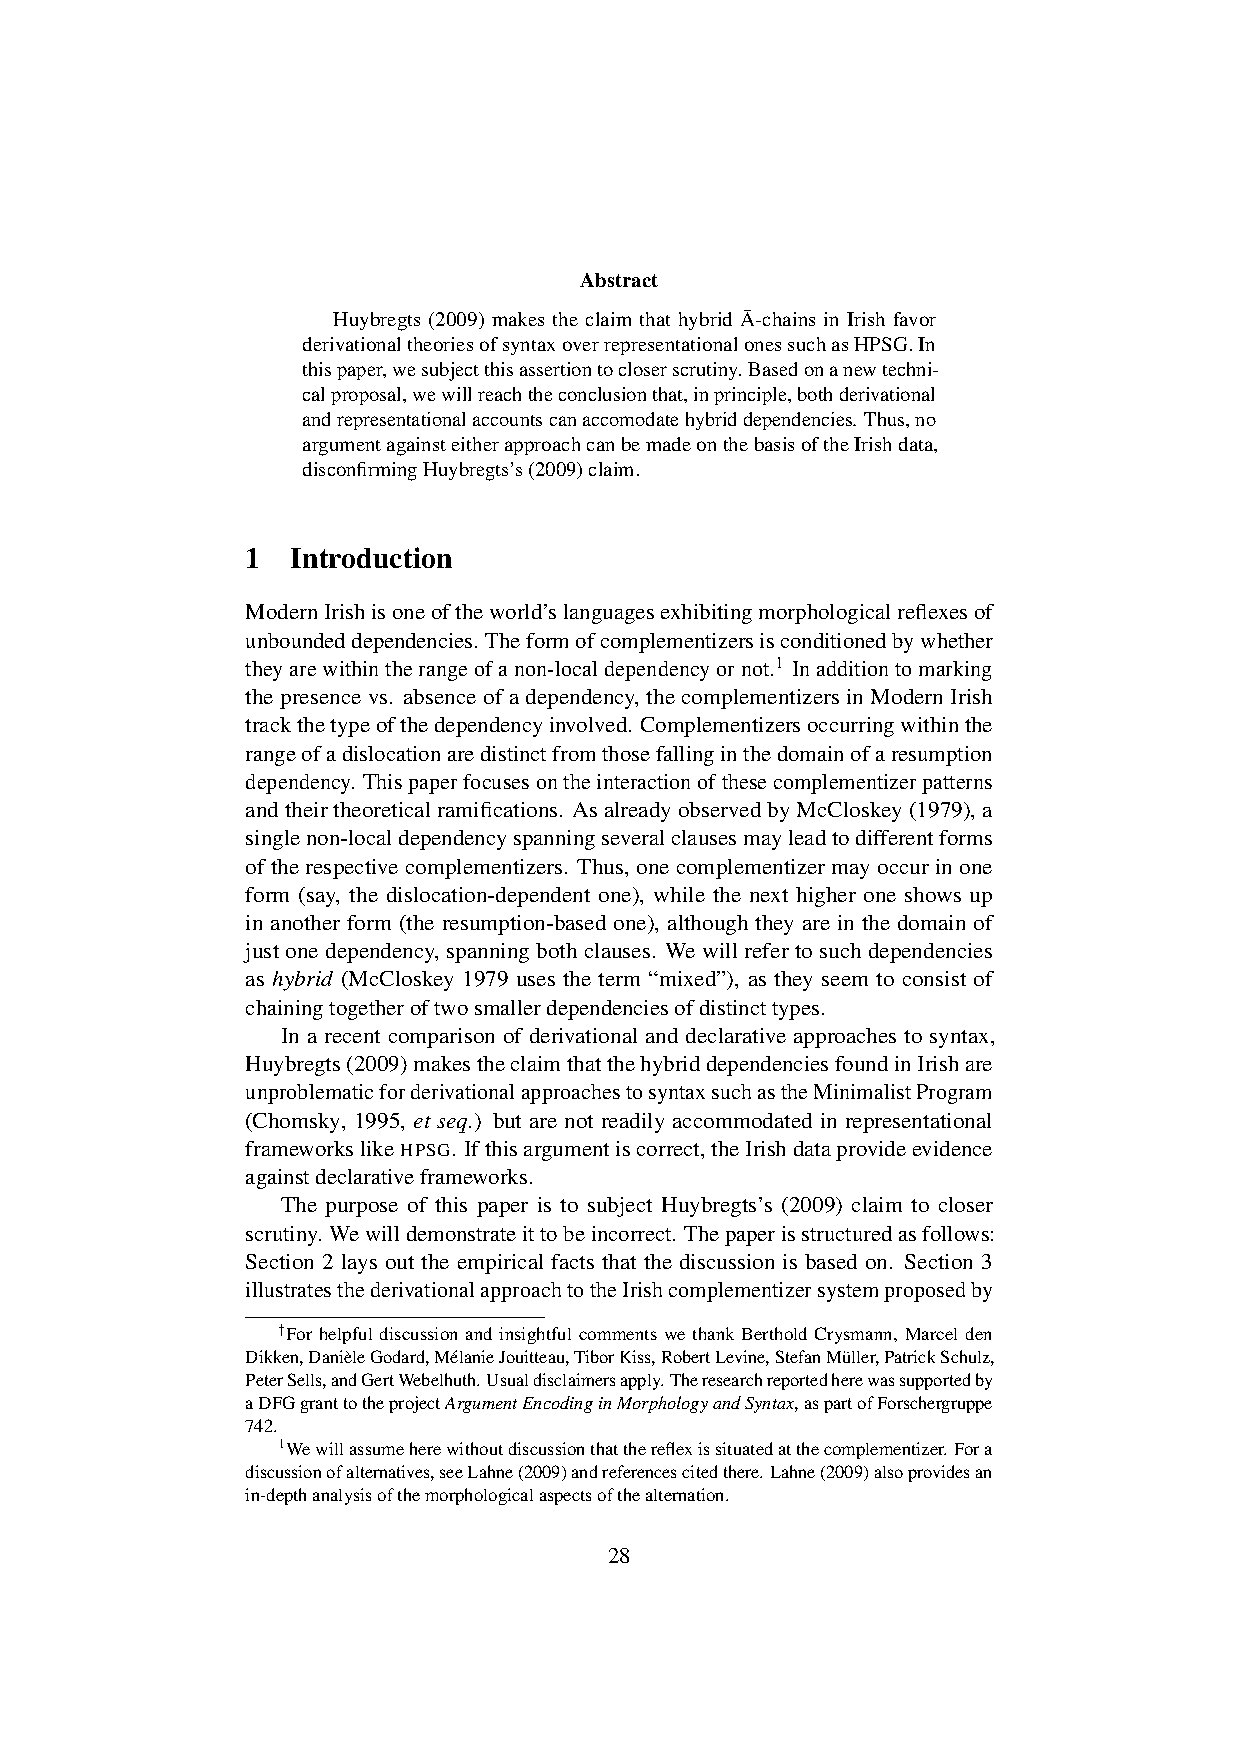
\includepdf[pages=-,pagecommand=\thispagestyle{plain}]{Includes/ahhkm.pdf}
        \setcounter{page}{47}
        \phantomsection
        \addcontentsline{toc}{section}{Doug Arnold, Robert D. Borsley: Auxiliary-Stranding Relative Clauses}
\thispagestyle{empty}

\begin{center}
  {\huge\bfseries Auxiliary-Stranding Relative Clauses\par}

  \bigskip

~\\
\begingroup
\setlength{\leftskip}{0pt plus 1fill}
\setlength{\rightskip}{0pt plus 1fill}
\setlength{\parindent}{0pt}
\setlength{\parfillskip}{0pt}
  \formatauthor{Doug Arnold}{\begin{tabular}{@{}c@{}}University of Essex\end{tabular}}
\formatauthor{Robert D. Borsley}{\begin{tabular}{@{}c@{}}University of Essex\end{tabular}}

\par\endgroup

  \vspace*{8ex}

  Proceedings of the 17th International Conference on\par Head-Driven Phrase Structure Grammar

  \bigskip

  Universit{\'e} Paris Diderot, Paris 7, France

  \medskip

  Stefan Müller (Editor)

  \medskip

  2010

  \medskip

  CSLI Publications

  \medskip

  pages 47--67

  \medskip

  \url{http://csli-publications.stanford.edu/HPSG/2010}
\end{center}
\vfill

\noindent



\vfill
\noindent
% APA Style
Arnold, Doug, \& Borsley, Robert D. 2010. Auxiliary-Stranding Relative Clauses. In Müller, Stefan (Ed.), \emph{{Proceedings of the 17th International Conference on Head-Driven Phrase Structure Grammar, Universit{\'e} Paris Diderot, Paris 7, France}}, 47--67. Stanford,
CA: CSLI Publications. \hfill\href{http://creativecommons.org/licenses/by/4.0/}{\includegraphics[height=.75em]{Includes/ccby.eps}}

\newpage
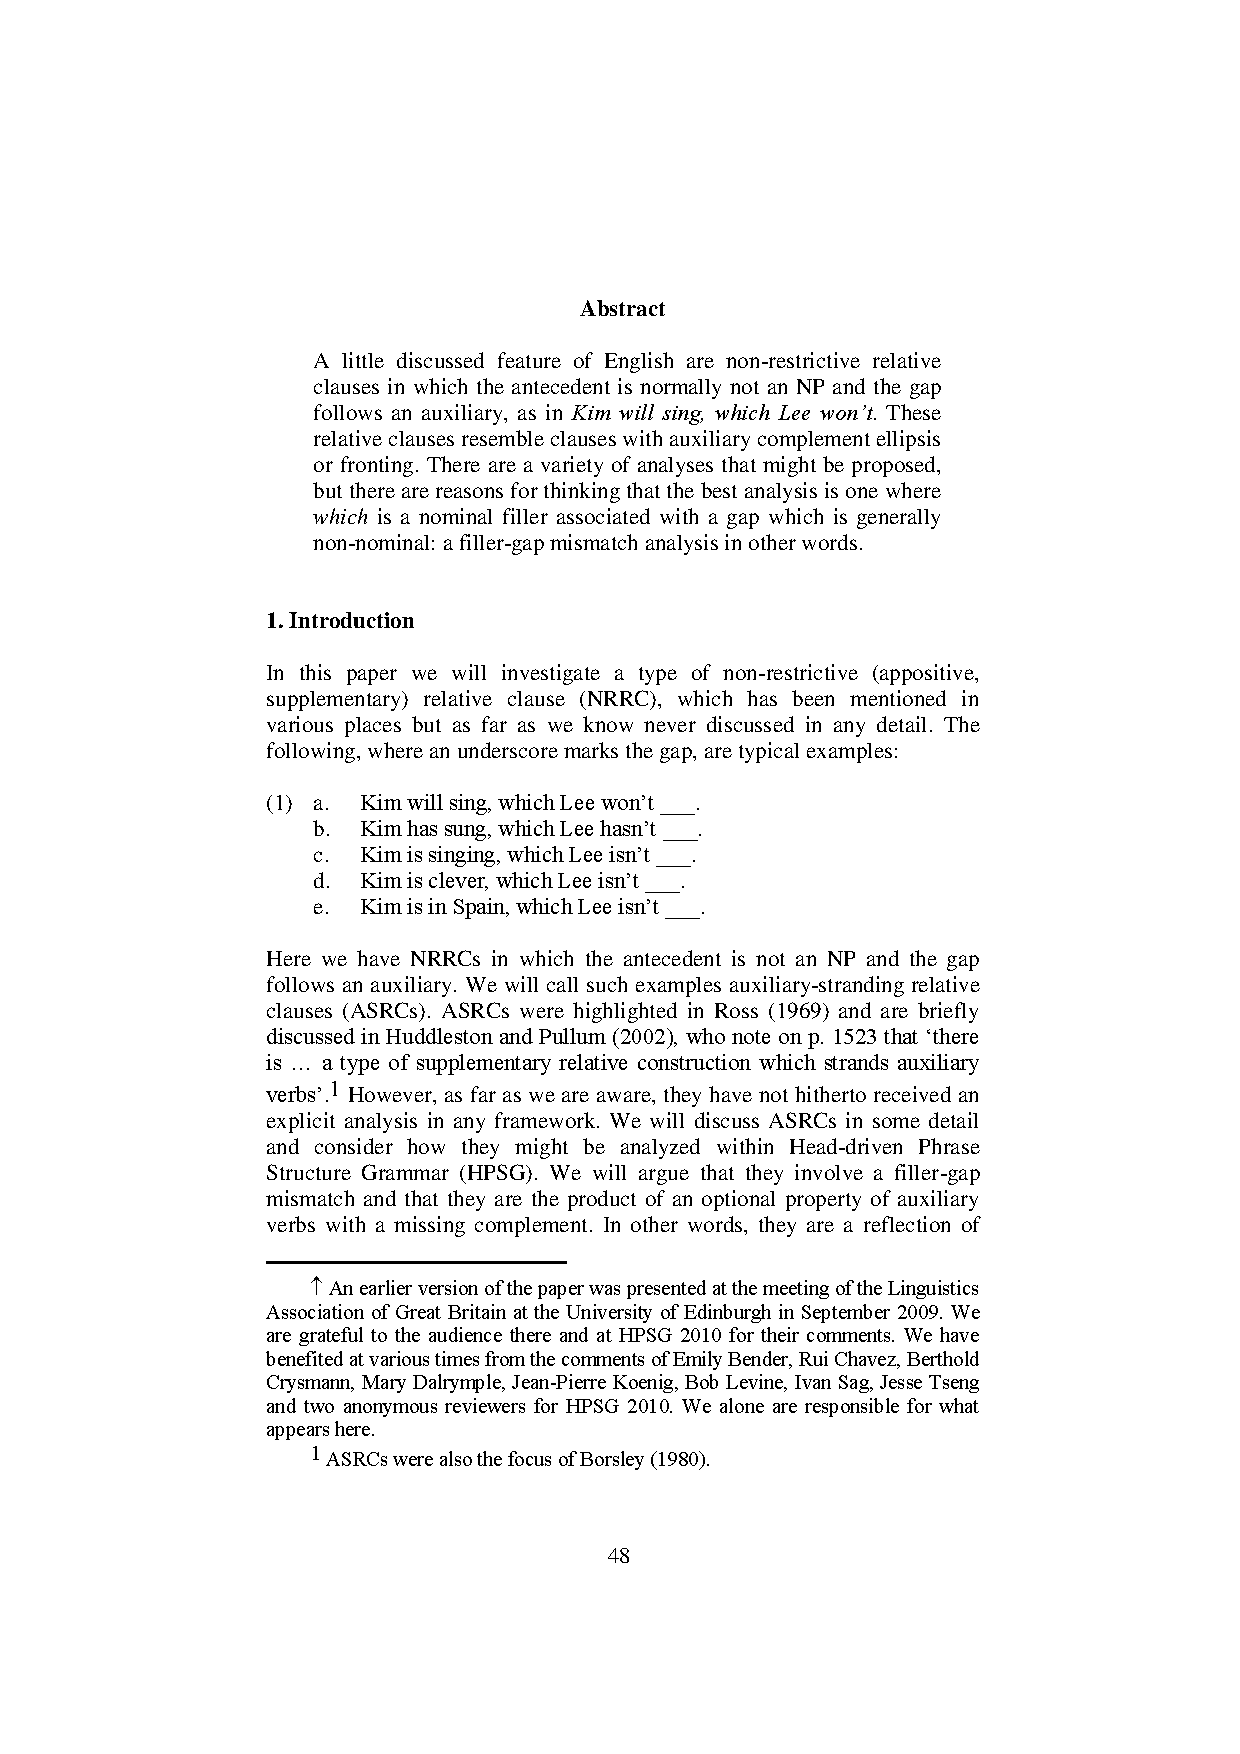
\includepdf[pages=-,pagecommand=\thispagestyle{plain}]{Includes/arnold-borsley.pdf}
        \setcounter{page}{68}
        \phantomsection
        \addcontentsline{toc}{section}{Felix Bildhauer, Philippa Cook: German Multiple Fronting and Expected Topic-Hood}
\thispagestyle{empty}

\begin{center}
  {\huge\bfseries German Multiple Fronting and Expected Topic-Hood\par}

  \bigskip

~\\
\begingroup
\setlength{\leftskip}{0pt plus 1fill}
\setlength{\rightskip}{0pt plus 1fill}
\setlength{\parindent}{0pt}
\setlength{\parfillskip}{0pt}
  \formatauthor{Felix Bildhauer}{\begin{tabular}{@{}c@{}}Freie Universität Berlin\end{tabular}}
\formatauthor{Philippa Cook}{\begin{tabular}{@{}c@{}}Freie Universität Berlin\end{tabular}}

\par\endgroup

  \vspace*{8ex}

  Proceedings of the 17th International Conference on\par Head-Driven Phrase Structure Grammar

  \bigskip

  Universit{\'e} Paris Diderot, Paris 7, France

  \medskip

  Stefan Müller (Editor)

  \medskip

  2010

  \medskip

  CSLI Publications

  \medskip

  pages 68--79

  \medskip

  \url{http://csli-publications.stanford.edu/HPSG/2010}
\end{center}
\vfill

\noindent



\vfill
\noindent
% APA Style
Bildhauer, Felix, \& Cook, Philippa. 2010. German Multiple Fronting and Expected Topic-Hood. In Müller, Stefan (Ed.), \emph{{Proceedings of the 17th International Conference on Head-Driven Phrase Structure Grammar, Universit{\'e} Paris Diderot, Paris 7, France}}, 68--79. Stanford,
CA: CSLI Publications. \hfill\href{http://creativecommons.org/licenses/by/4.0/}{\includegraphics[height=.75em]{Includes/ccby.eps}}

\newpage
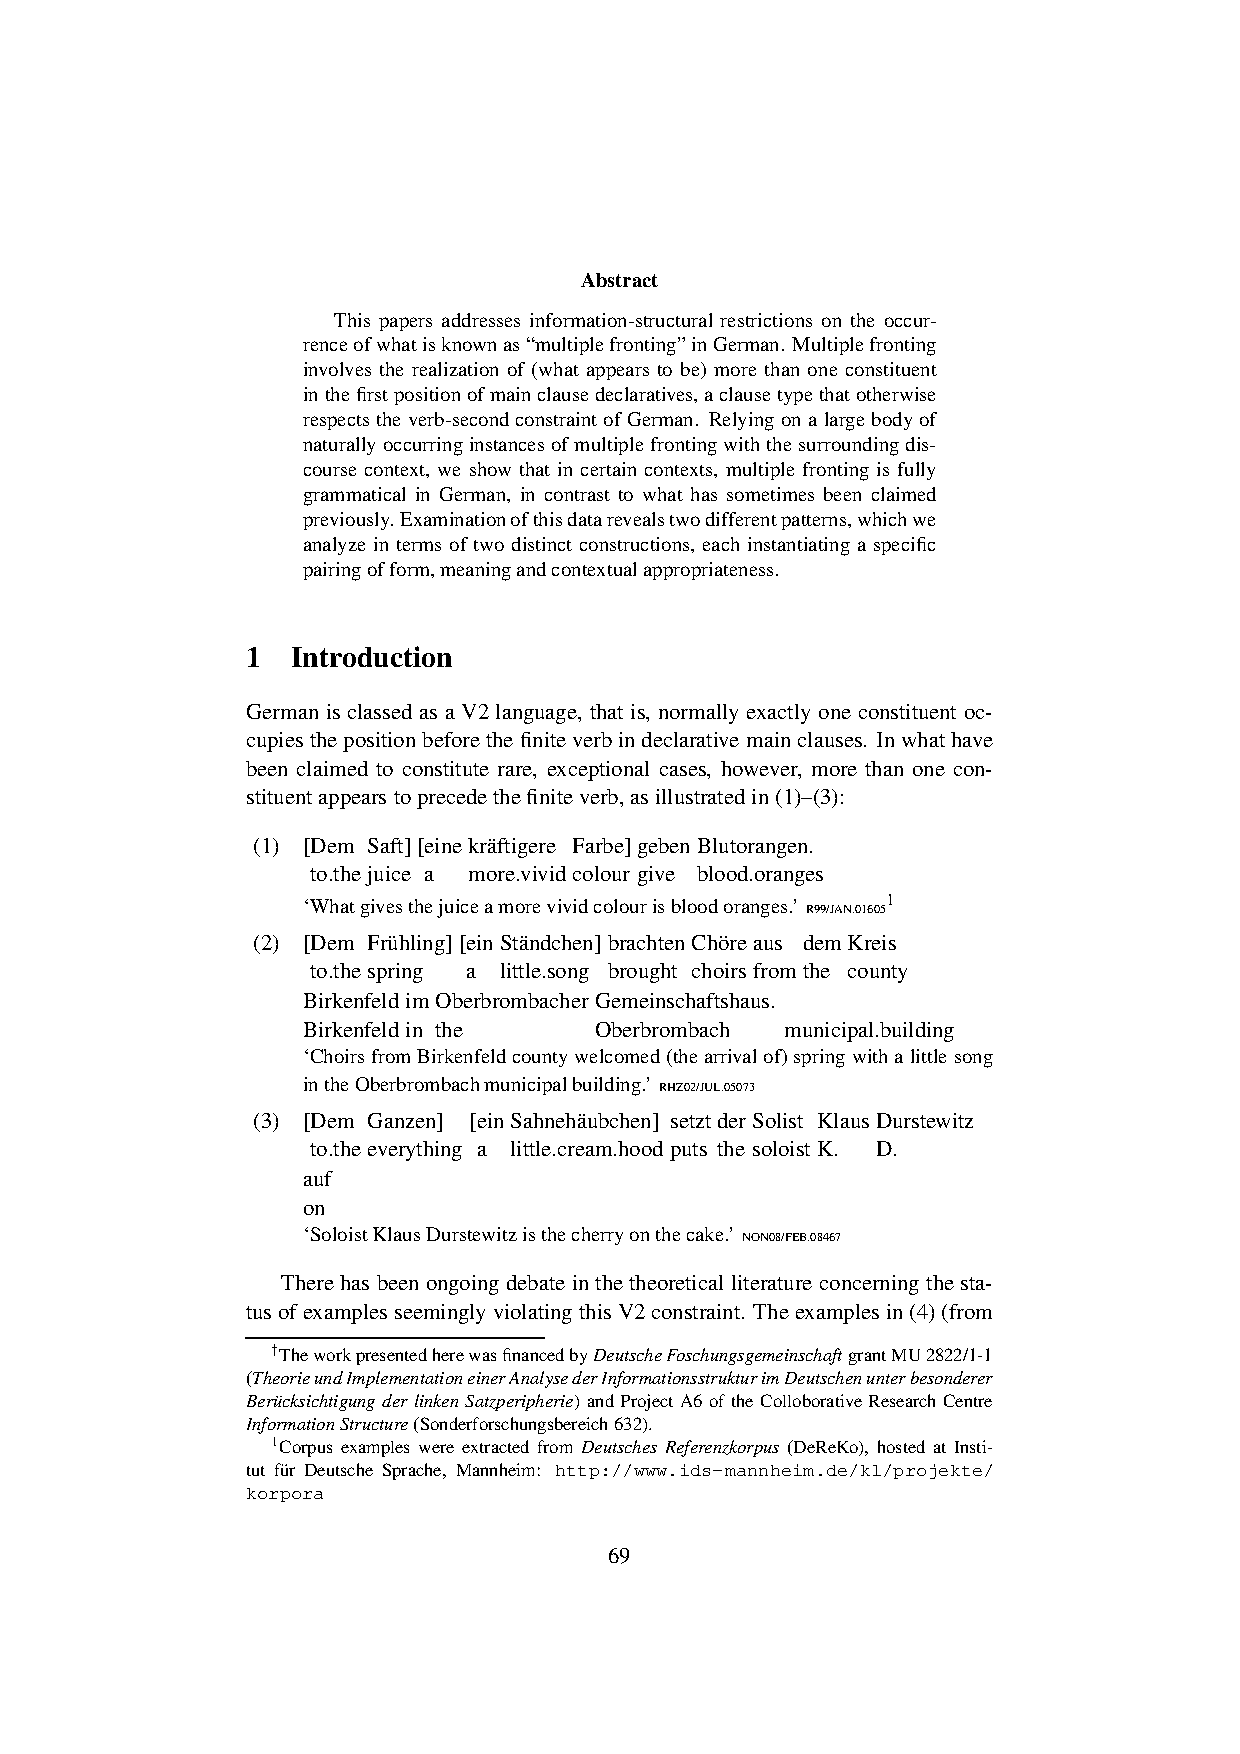
\includepdf[pages=-,pagecommand=\thispagestyle{plain}]{Includes/bildhauer-cook.pdf}
        \setcounter{page}{80}
        \phantomsection
        \addcontentsline{toc}{section}{Robert D Borsley: An HPSG Approach to Welsh Unbounded Dependencies}
\thispagestyle{empty}

\begin{center}
  {\huge\bfseries An HPSG Approach to Welsh Unbounded Dependencies\par}

  \bigskip

~\\
\begingroup
\setlength{\leftskip}{0pt plus 1fill}
\setlength{\rightskip}{0pt plus 1fill}
\setlength{\parindent}{0pt}
\setlength{\parfillskip}{0pt}
  \formatauthor{Robert D Borsley}{\begin{tabular}{@{}c@{}}University of Essex\end{tabular}}

\par\endgroup

  \vspace*{8ex}

  Proceedings of the 17th International Conference on\par Head-Driven Phrase Structure Grammar

  \bigskip

  Universit{\'e} Paris Diderot, Paris 7, France

  \medskip

  Stefan Müller (Editor)

  \medskip

  2010

  \medskip

  CSLI Publications

  \medskip

  pages 80--100

  \medskip

  \url{http://csli-publications.stanford.edu/HPSG/2010}
\end{center}
\vfill

\noindent



\vfill
\noindent
% APA Style
Borsley, Robert D. 2010. An HPSG Approach to Welsh Unbounded Dependencies. In Müller, Stefan (Ed.), \emph{{Proceedings of the 17th International Conference on Head-Driven Phrase Structure Grammar, Universit{\'e} Paris Diderot, Paris 7, France}}, 80--100. Stanford,
CA: CSLI Publications. \hfill\href{http://creativecommons.org/licenses/by/4.0/}{\includegraphics[height=.75em]{Includes/ccby.eps}}

\newpage
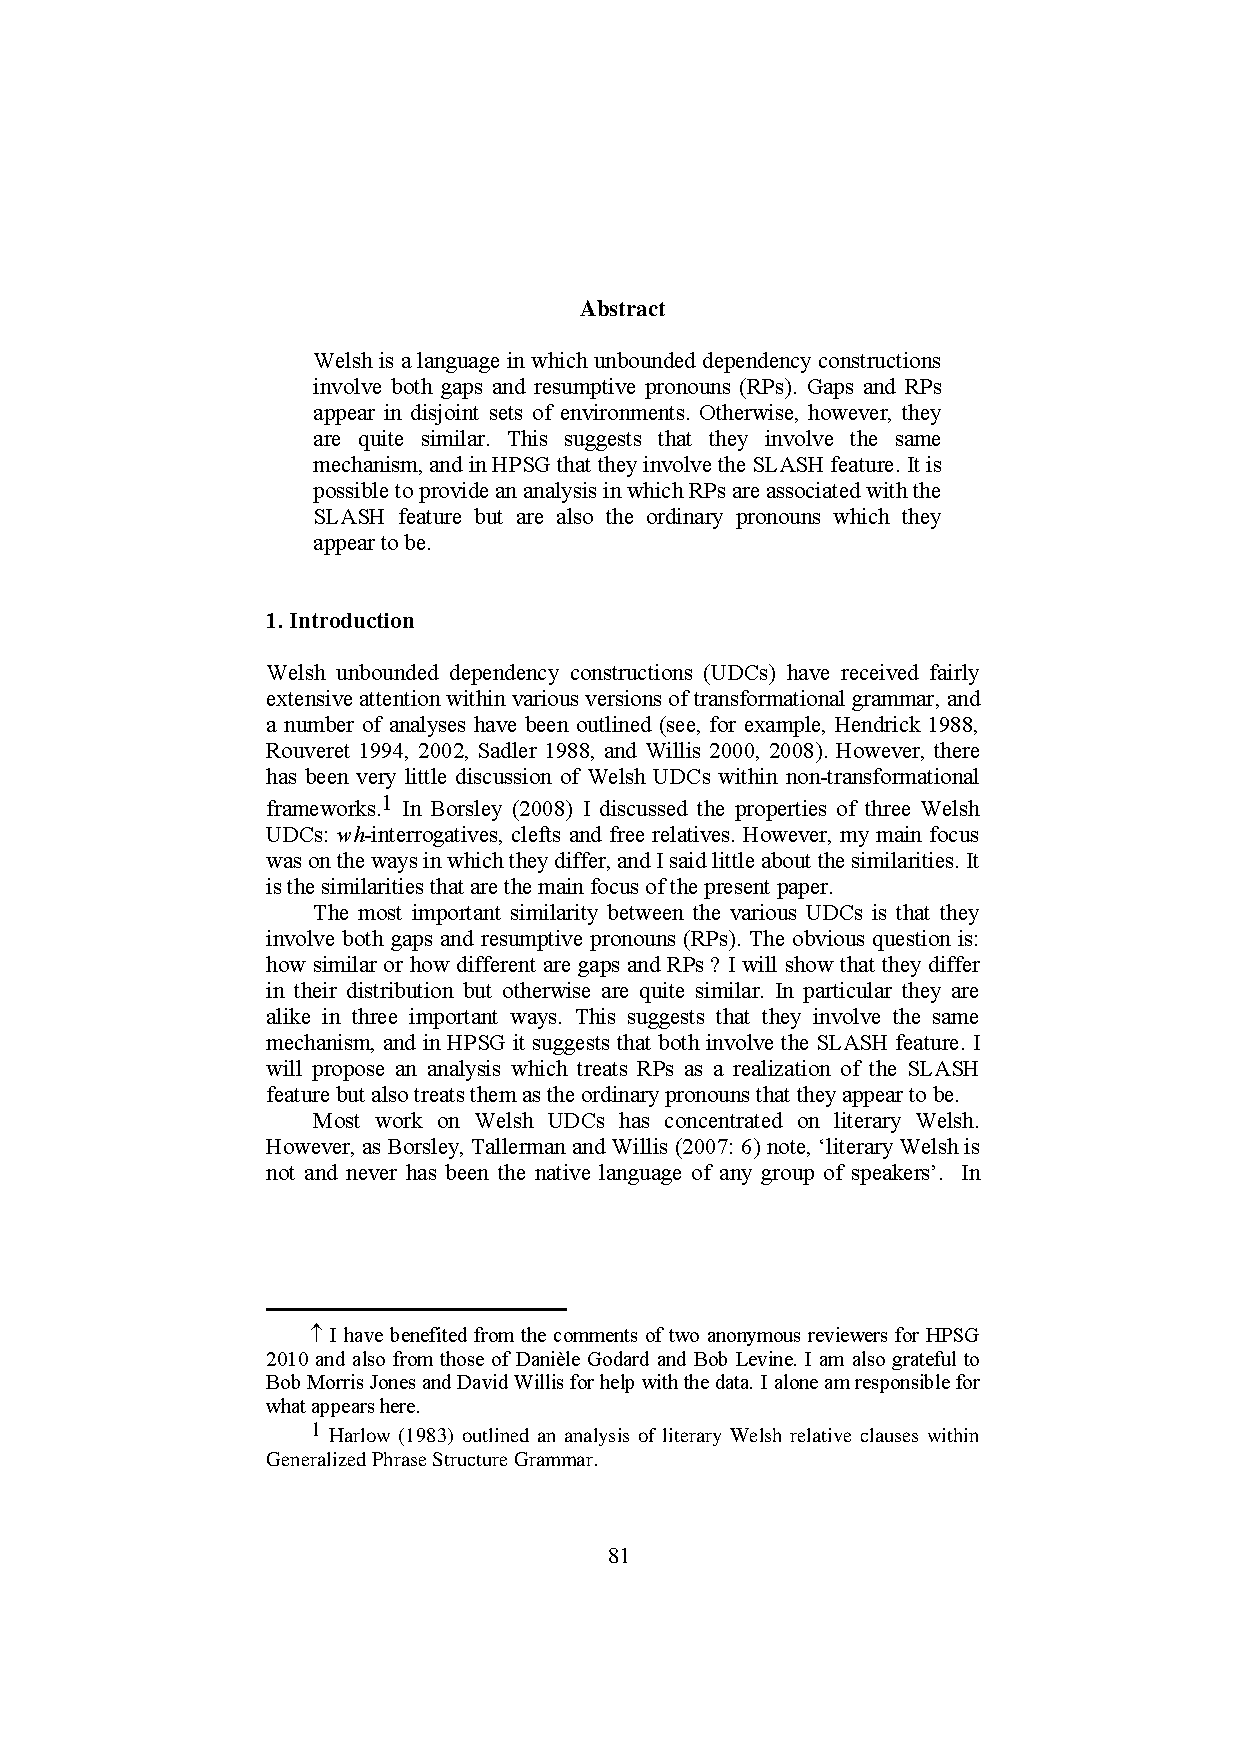
\includepdf[pages=-,pagecommand=\thispagestyle{plain}]{Includes/borsley.pdf}
        \setcounter{page}{101}
        \phantomsection
        \addcontentsline{toc}{section}{Rui P. Chaves: On the Syntax and Semantics of \emph{vice versa}}
\thispagestyle{empty}

\begin{center}
  {\huge\bfseries On the Syntax and Semantics of \emph{vice versa}\par}

  \bigskip

~\\
\begingroup
\setlength{\leftskip}{0pt plus 1fill}
\setlength{\rightskip}{0pt plus 1fill}
\setlength{\parindent}{0pt}
\setlength{\parfillskip}{0pt}
  \formatauthor{Rui P. Chaves}{\begin{tabular}{@{}c@{}}University at Buffalo\end{tabular}}

\par\endgroup

  \vspace*{8ex}

  Proceedings of the 17th International Conference on\par Head-Driven Phrase Structure Grammar

  \bigskip

  Universit{\'e} Paris Diderot, Paris 7, France

  \medskip

  Stefan Müller (Editor)

  \medskip

  2010

  \medskip

  CSLI Publications

  \medskip

  pages 101--121

  \medskip

  \url{http://csli-publications.stanford.edu/HPSG/2010}
\end{center}
\vfill

\noindent



\vfill
\noindent
% APA Style
Chaves, Rui P. 2010. On the Syntax and Semantics of \emph{vice versa}. In Müller, Stefan (Ed.), \emph{{Proceedings of the 17th International Conference on Head-Driven Phrase Structure Grammar, Universit{\'e} Paris Diderot, Paris 7, France}}, 101--121. Stanford,
CA: CSLI Publications. \hfill\href{http://creativecommons.org/licenses/by/4.0/}{\includegraphics[height=.75em]{Includes/ccby.eps}}

\newpage
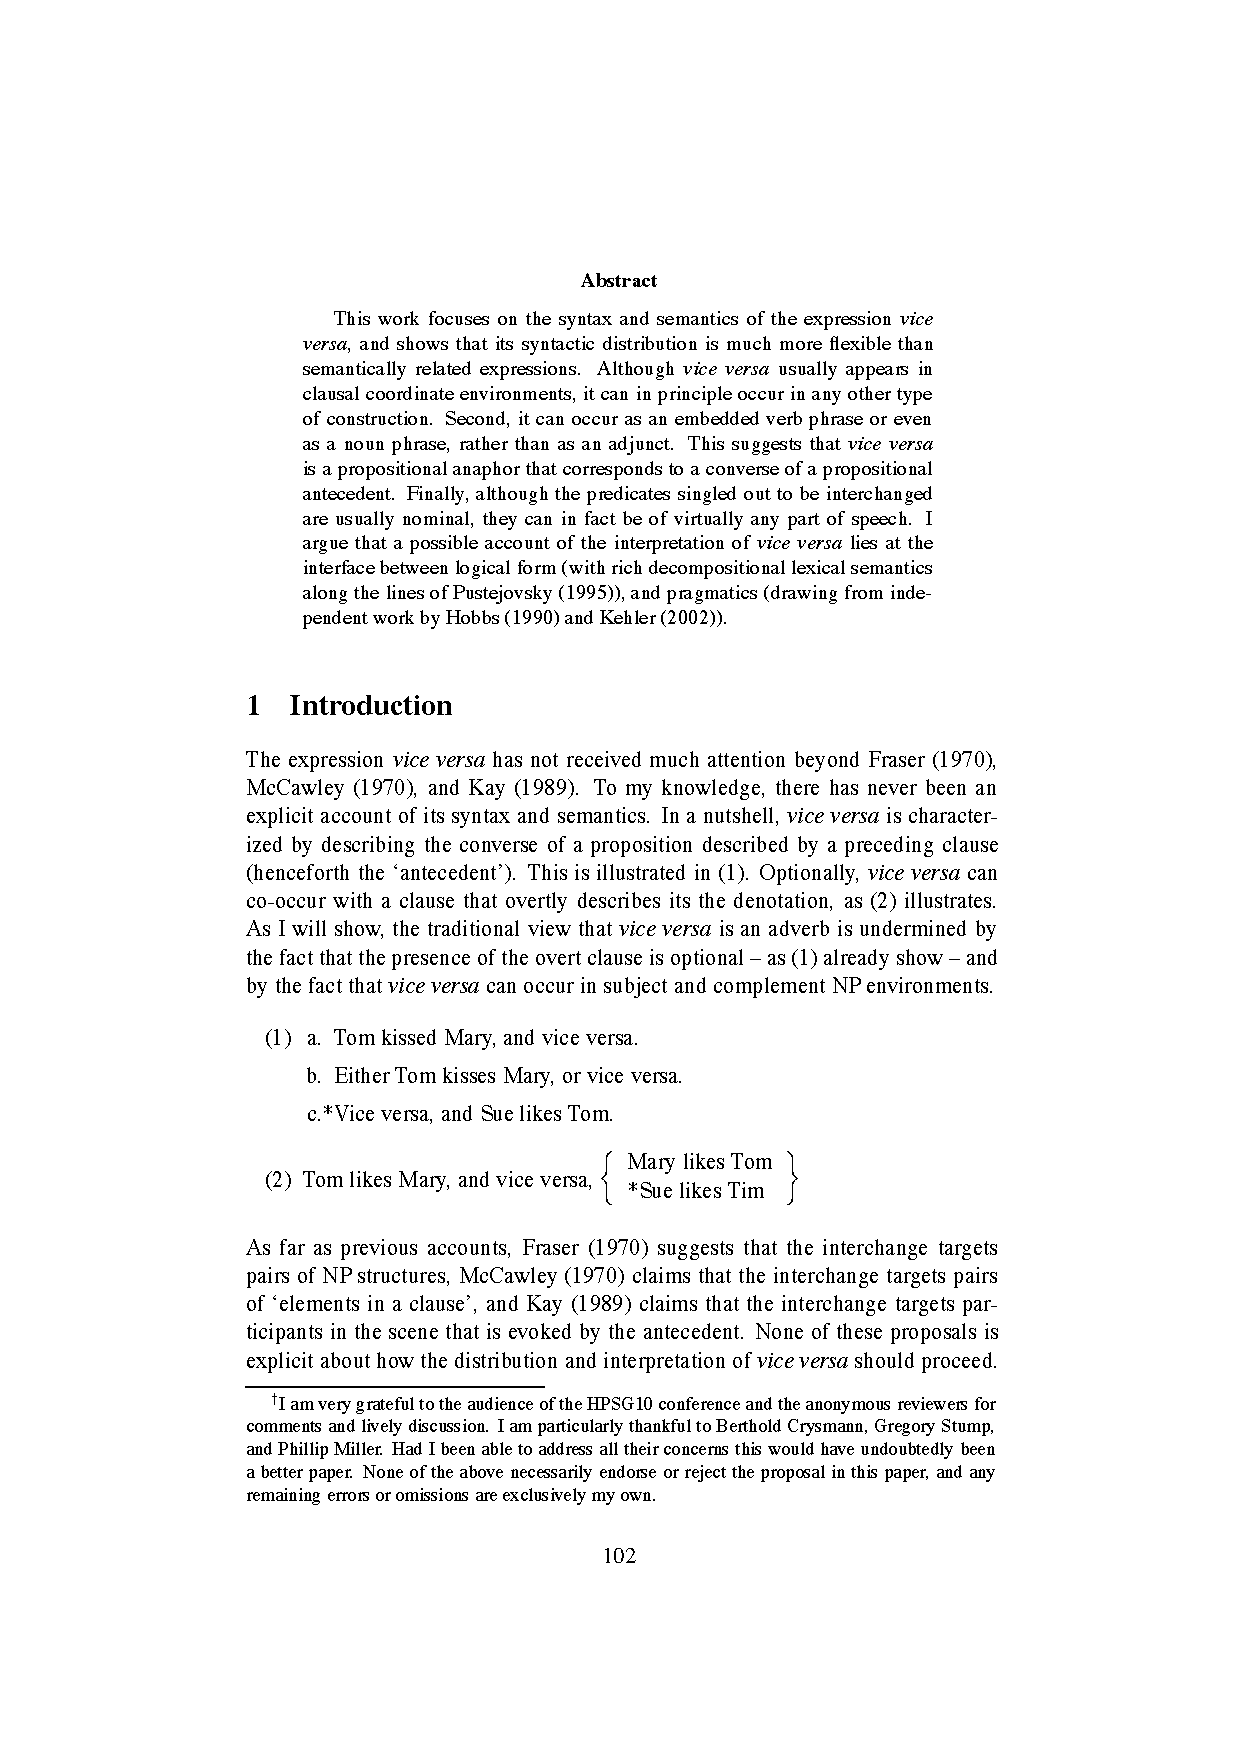
\includepdf[pages=-,pagecommand=\thispagestyle{plain}]{Includes/chaves.pdf}
        \setcounter{page}{122}
        \phantomsection
        \addcontentsline{toc}{section}{Philippa Cook, Bjarne {\O}rsnes: Coherence with adjectives in German}
\thispagestyle{empty}

\begin{center}
  {\huge\bfseries Coherence with adjectives in German\par}

  \bigskip

~\\
\begingroup
\setlength{\leftskip}{0pt plus 1fill}
\setlength{\rightskip}{0pt plus 1fill}
\setlength{\parindent}{0pt}
\setlength{\parfillskip}{0pt}
  \formatauthor{Philippa Cook}{\begin{tabular}{@{}c@{}}Freie Universität Berlin\end{tabular}}
\formatauthor{Bjarne Ørsnes}{\begin{tabular}{@{}c@{}}Freie Universität Berlin\end{tabular}}

\par\endgroup

  \vspace*{8ex}

  Proceedings of the 17th International Conference on\par Head-Driven Phrase Structure Grammar

  \bigskip

  Universit{\'e} Paris Diderot, Paris 7, France

  \medskip

  Stefan Müller (Editor)

  \medskip

  2010

  \medskip

  CSLI Publications

  \medskip

  pages 122--142

  \medskip

  \url{http://csli-publications.stanford.edu/HPSG/2010}
\end{center}
\vfill

\noindent



\vfill
\noindent
% APA Style
Cook, Philippa, \& Ørsnes, Bjarne. 2010. Coherence with adjectives in German. In Müller, Stefan (Ed.), \emph{{Proceedings of the 17th International Conference on Head-Driven Phrase Structure Grammar, Universit{\'e} Paris Diderot, Paris 7, France}}, 122--142. Stanford,
CA: CSLI Publications. \hfill\href{http://creativecommons.org/licenses/by/4.0/}{\includegraphics[height=.75em]{Includes/ccby.eps}}

\newpage
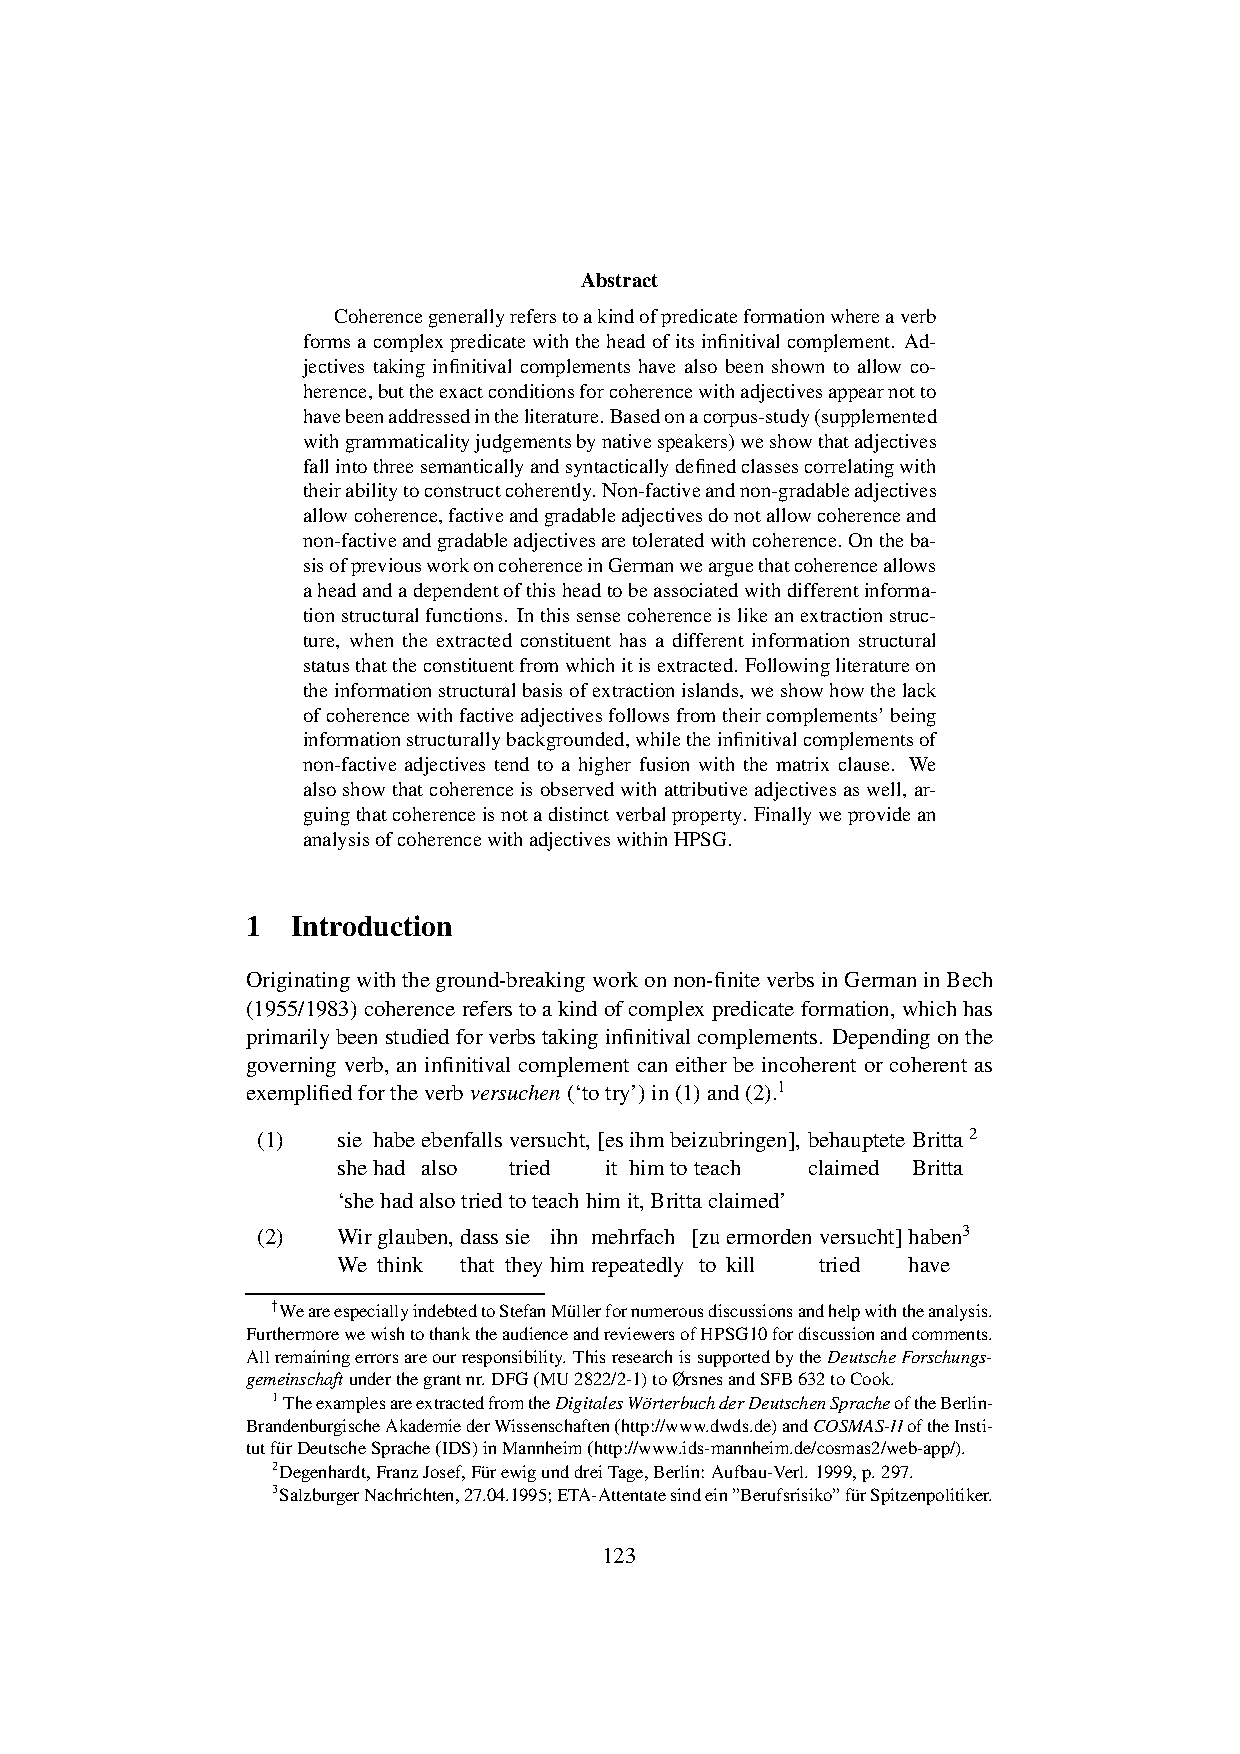
\includepdf[pages=-,pagecommand=\thispagestyle{plain}]{Includes/cook-oersnes.pdf}
        \setcounter{page}{143}
        \phantomsection
        \addcontentsline{toc}{section}{Barbara Hemforth, Michel Fayol, S{\'e}bastien Pacton: Usage-based Preferences in Written Sentence
 Production: The Role of Local and Global Statistics}
\thispagestyle{empty}

\begin{center}
  {\huge\bfseries Usage-based Preferences in Written Sentence
 Production: The Role of Local and Global Statistics\par}

  \bigskip

~\\
\begingroup
\setlength{\leftskip}{0pt plus 1fill}
\setlength{\rightskip}{0pt plus 1fill}
\setlength{\parindent}{0pt}
\setlength{\parfillskip}{0pt}
  \formatauthor{Barbara Hemforth}{\begin{tabular}{@{}c@{}}LPNCog, CNRS, IUPPD-Université Paris-Descartes\end{tabular}}
\formatauthor{Michel Fayol}{\begin{tabular}{@{}c@{}}LAPSCO, CNRS, Université Blaise Pascal, Clermont-Ferrand\end{tabular}}
\formatauthor{Sébastien Pacton}{\begin{tabular}{@{}c@{}}LPNCog, CNRS, IUPPD-Université Paris-Descartes\end{tabular}}

\par\endgroup

  \vspace*{8ex}

  Proceedings of the 17th International Conference on\par Head-Driven Phrase Structure Grammar

  \bigskip

  Universit{\'e} Paris Diderot, Paris 7, France

  \medskip

  Stefan Müller (Editor)

  \medskip

  2010

  \medskip

  CSLI Publications

  \medskip

  pages 143--157

  \medskip

  \url{http://csli-publications.stanford.edu/HPSG/2010}
\end{center}
\vfill

\noindent



\vfill
\noindent
% APA Style
Hemforth, Barbara, Fayol, Michel, \& Pacton, Sébastien. 2010. Usage-based Preferences in Written Sentence
 Production: The Role of Local and Global Statistics. In Müller, Stefan (Ed.), \emph{{Proceedings of the 17th International Conference on Head-Driven Phrase Structure Grammar, Universit{\'e} Paris Diderot, Paris 7, France}}, 143--157. Stanford,
CA: CSLI Publications. \hfill\href{http://creativecommons.org/licenses/by/4.0/}{\includegraphics[height=.75em]{Includes/ccby.eps}}

\newpage
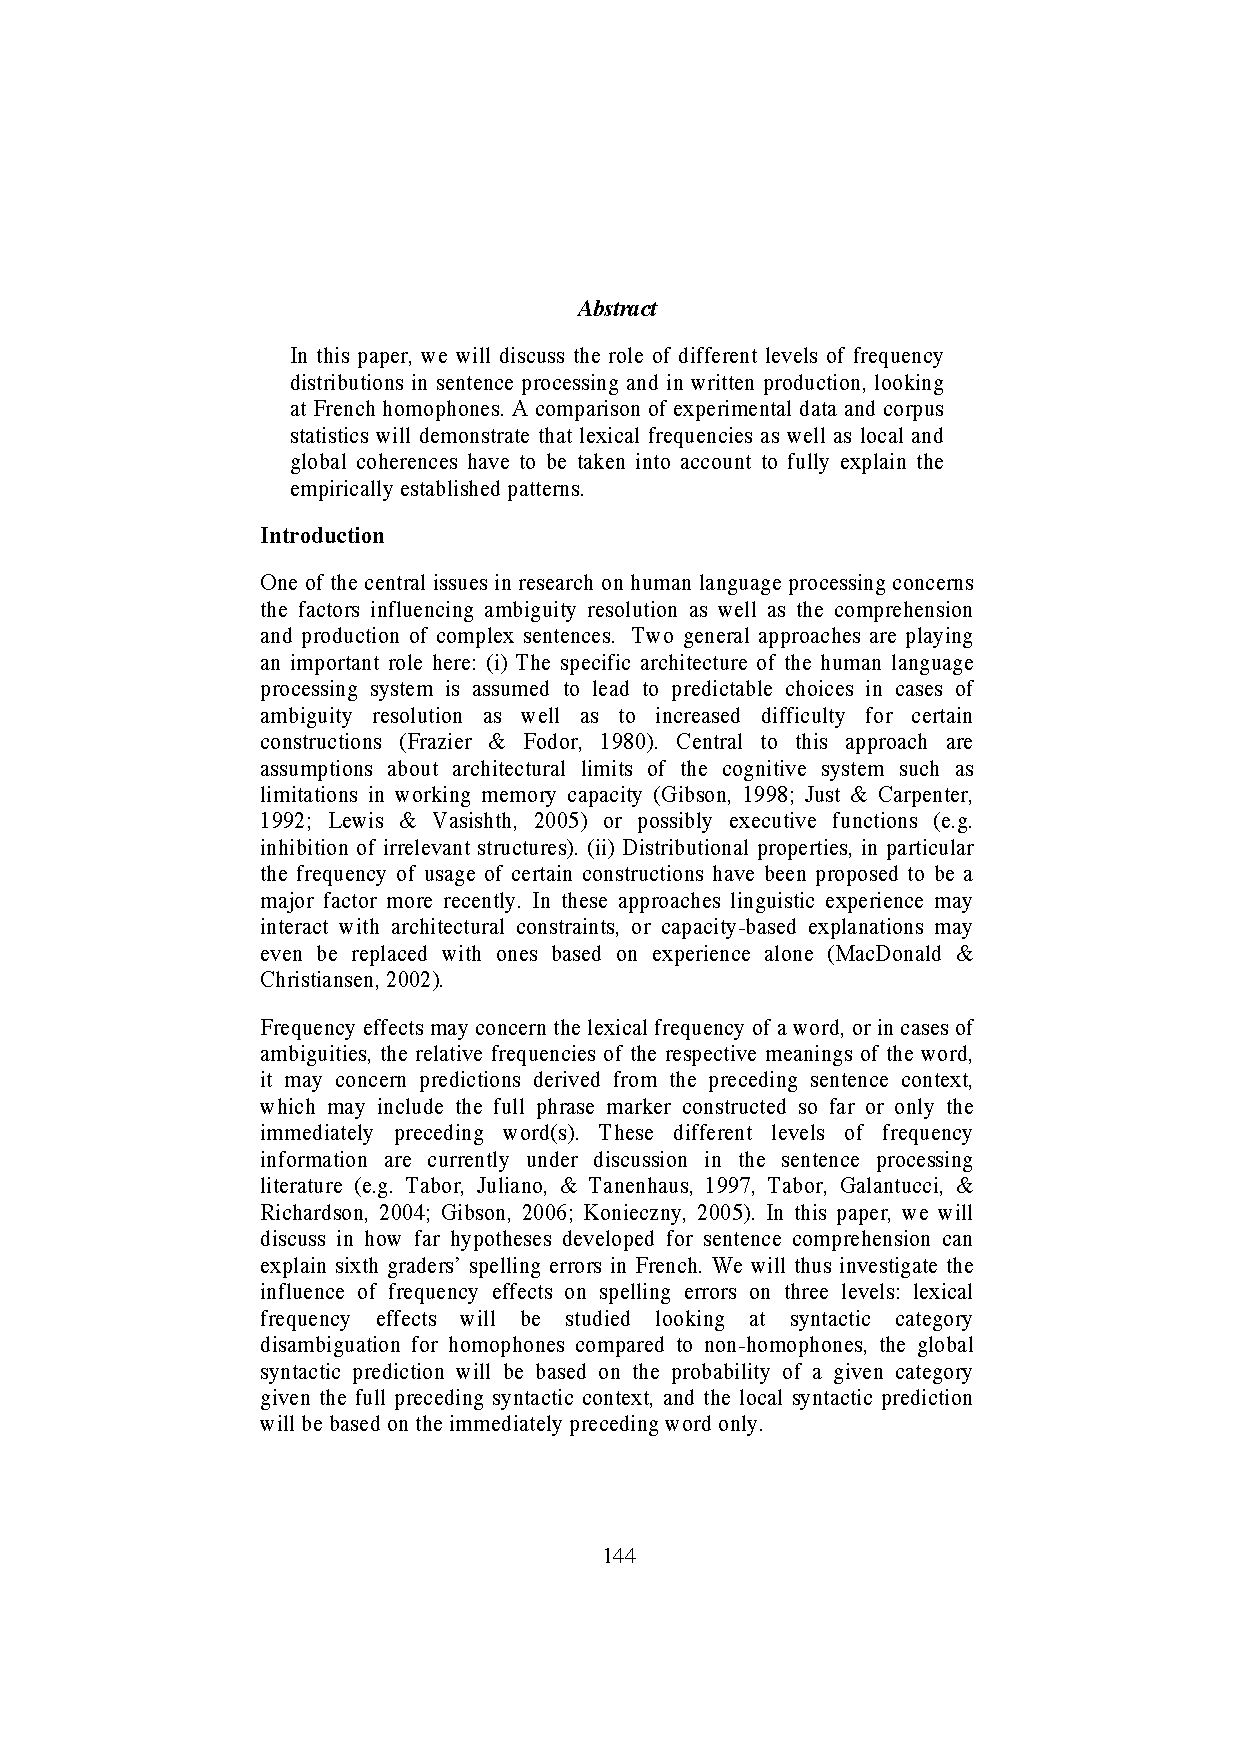
\includepdf[pages=-,pagecommand=\thispagestyle{plain}]{Includes/hfp.pdf}
        \setcounter{page}{158}
        \phantomsection
        \addcontentsline{toc}{section}{Md. Sadiqul Islam, Mahmudul Hasan Masum, Md. Shariful Islam Bhuyan, Reaz Ahmed: Arabic Nominals in HPSG: A Verbal Noun Perspective}
\thispagestyle{empty}

\begin{center}
  {\huge\bfseries Arabic Nominals in HPSG: A Verbal Noun Perspective\par}

  \bigskip

~\\
\begingroup
\setlength{\leftskip}{0pt plus 1fill}
\setlength{\rightskip}{0pt plus 1fill}
\setlength{\parindent}{0pt}
\setlength{\parfillskip}{0pt}
  \formatauthor{Md. Sadiqul Islam}{\begin{tabular}{@{}c@{}}Bangladesh University of Engineering and Technology, Dhaka\end{tabular}}
\formatauthor{Mahmudul Hasan Masum}{\begin{tabular}{@{}c@{}}Bangladesh University of Engineering and Technology, Dhaka\end{tabular}}
\formatauthor{Md. Shariful Islam Bhuyan}{\begin{tabular}{@{}c@{}}Bangladesh University of Engineering and Technology, Dhaka\end{tabular}}
\formatauthor{Reaz Ahmed}{\begin{tabular}{@{}c@{}}Bangladesh University of Engineering and Technology, Dhaka\end{tabular}}

\par\endgroup

  \vspace*{8ex}

  Proceedings of the 17th International Conference on\par Head-Driven Phrase Structure Grammar

  \bigskip

  Universit{\'e} Paris Diderot, Paris 7, France

  \medskip

  Stefan Müller (Editor)

  \medskip

  2010

  \medskip

  CSLI Publications

  \medskip

  pages 158--178

  \medskip

  \url{http://csli-publications.stanford.edu/HPSG/2010}
\end{center}
\vfill

\noindent



\vfill
\noindent
% APA Style
Islam, Md. Sadiqul, Masum, Mahmudul Hasan, Bhuyan, Md. Shariful Islam, \& Ahmed, Reaz. 2010. Arabic Nominals in HPSG: A Verbal Noun Perspective. In Müller, Stefan (Ed.), \emph{{Proceedings of the 17th International Conference on Head-Driven Phrase Structure Grammar, Universit{\'e} Paris Diderot, Paris 7, France}}, 158--178. Stanford,
CA: CSLI Publications. \hfill\href{http://creativecommons.org/licenses/by/4.0/}{\includegraphics[height=.75em]{Includes/ccby.eps}}

\newpage
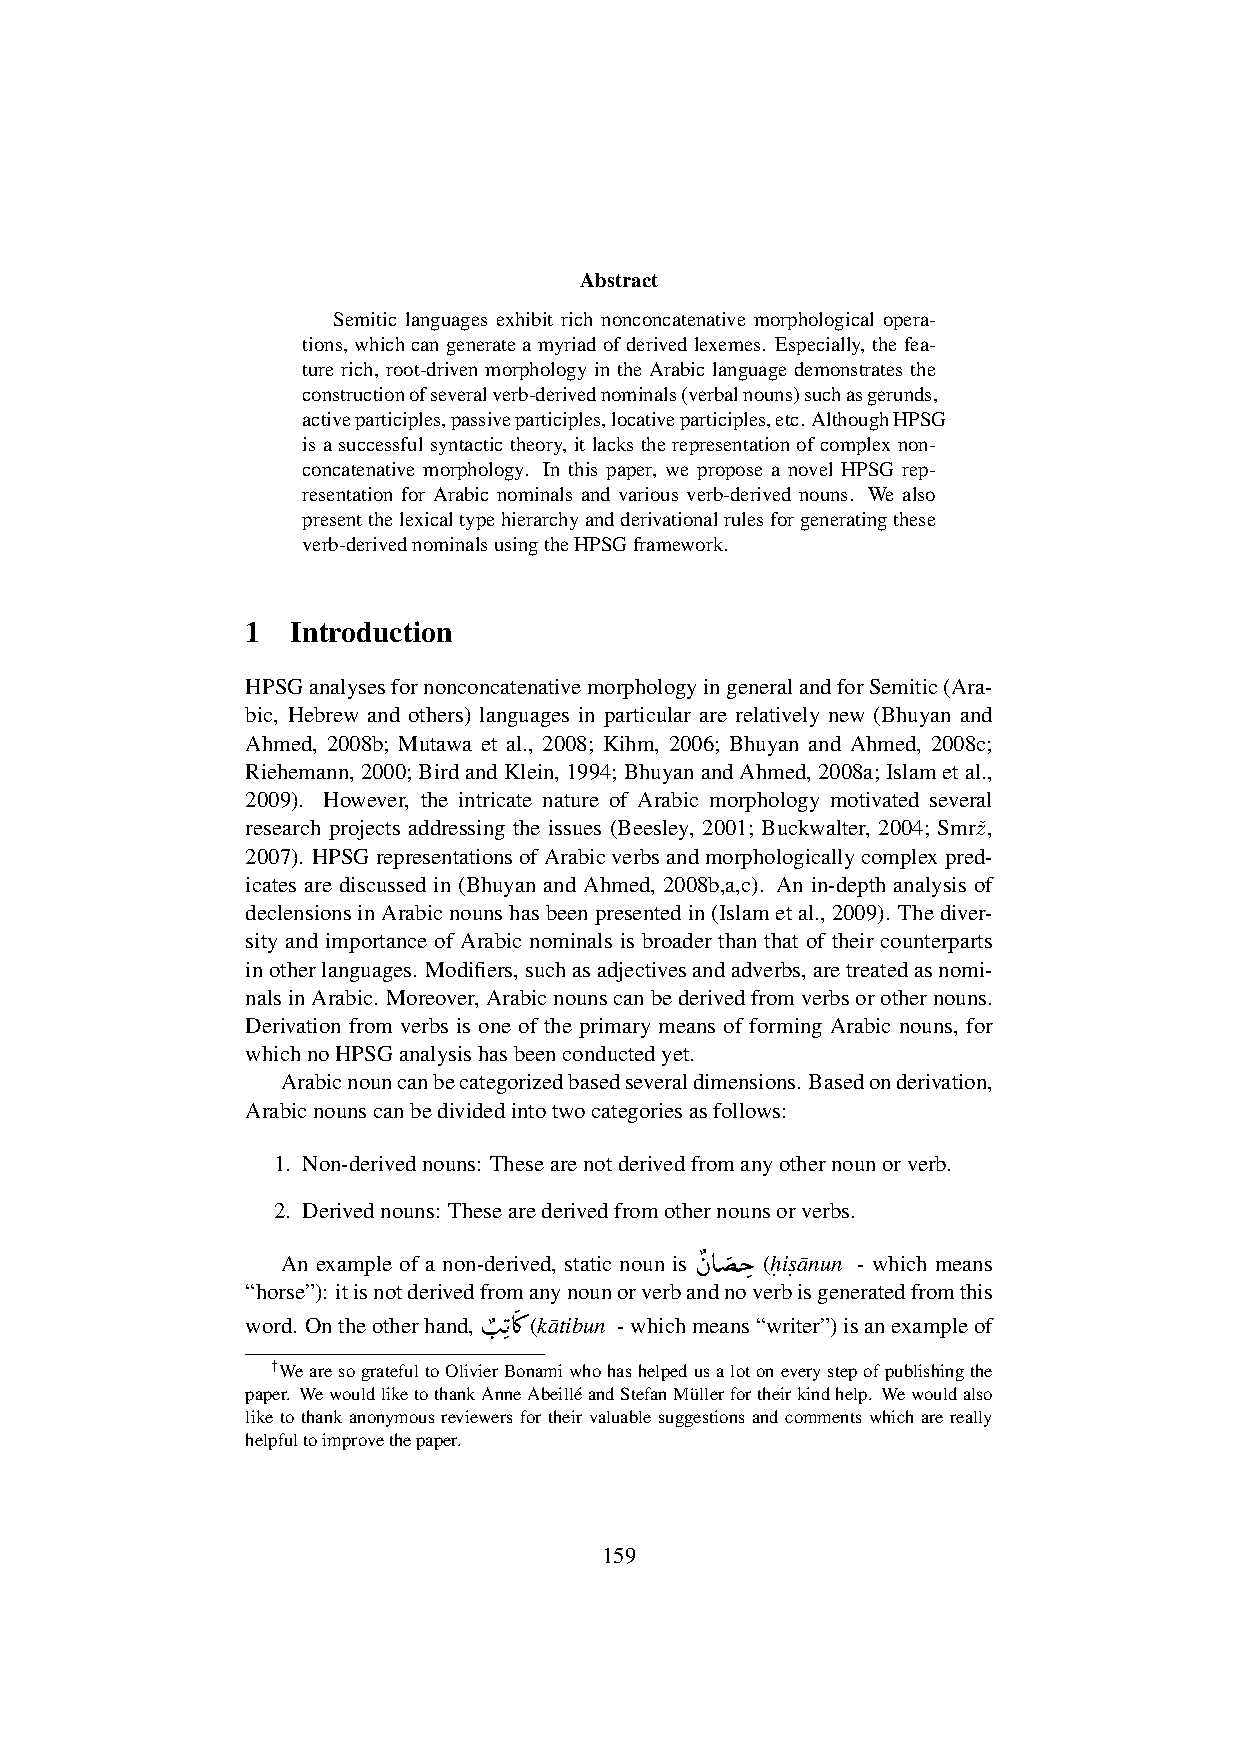
\includepdf[pages=-,pagecommand=\thispagestyle{plain}]{Includes/imba.pdf}
        \setcounter{page}{179}
        \phantomsection
        \addcontentsline{toc}{section}{Jong-Bok Kim, Jaehyung Yang, Sanghoun Song: Korean Comparative Constructions: A Constraint-Based Approach and Computational Implementation}
\thispagestyle{empty}

\begin{center}
  {\huge\bfseries Korean Comparative Constructions: A Constraint-Based Approach and Computational Implementation\par}

  \bigskip

~\\
\begingroup
\setlength{\leftskip}{0pt plus 1fill}
\setlength{\rightskip}{0pt plus 1fill}
\setlength{\parindent}{0pt}
\setlength{\parfillskip}{0pt}
  \formatauthor{Jong-Bok Kim}{\begin{tabular}{@{}c@{}}Kyung Hee\end{tabular}}
\formatauthor{Jaehyung Yang}{\begin{tabular}{@{}c@{}}Kangnam\end{tabular}}
\formatauthor{Sanghoun Song}{\begin{tabular}{@{}c@{}}University of Washington\end{tabular}}

\par\endgroup

  \vspace*{8ex}

  Proceedings of the 17th International Conference on\par Head-Driven Phrase Structure Grammar

  \bigskip

  Universit{\'e} Paris Diderot, Paris 7, France

  \medskip

  Stefan Müller (Editor)

  \medskip

  2010

  \medskip

  CSLI Publications

  \medskip

  pages 179--190

  \medskip

  \url{http://csli-publications.stanford.edu/HPSG/2010}
\end{center}
\vfill

\noindent



\vfill
\noindent
% APA Style
Kim, Jong-Bok, Yang, Jaehyung, \& Song, Sanghoun. 2010. Korean Comparative Constructions: A Constraint-Based Approach and Computational Implementation. In Müller, Stefan (Ed.), \emph{{Proceedings of the 17th International Conference on Head-Driven Phrase Structure Grammar, Universit{\'e} Paris Diderot, Paris 7, France}}, 179--190. Stanford,
CA: CSLI Publications. \hfill\href{http://creativecommons.org/licenses/by/4.0/}{\includegraphics[height=.75em]{Includes/ccby.eps}}

\newpage
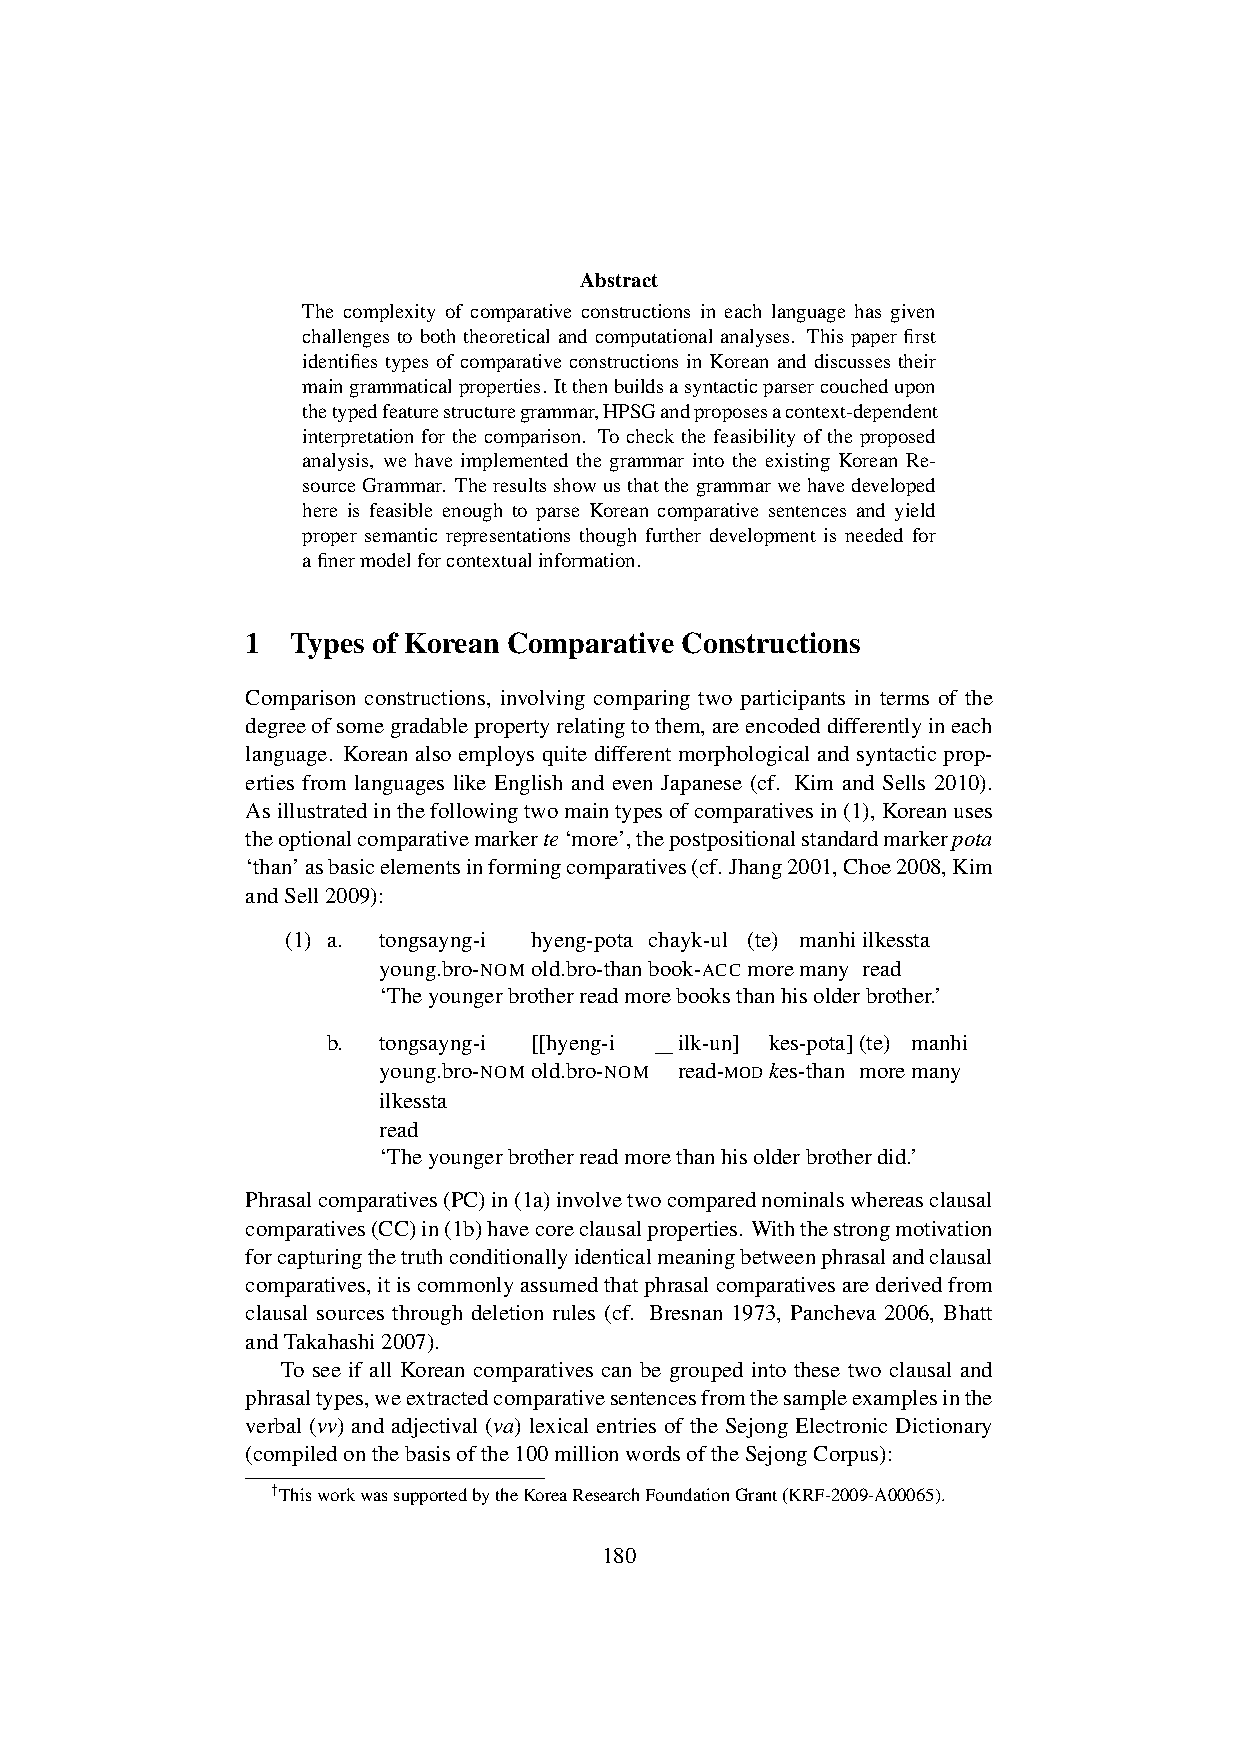
\includepdf[pages=-,pagecommand=\thispagestyle{plain}]{Includes/kys.pdf}
        \setcounter{page}{191}
        \phantomsection
        \addcontentsline{toc}{section}{Manfred Sailer: The Family of English Cognate Object Constructions}
\thispagestyle{empty}

\begin{center}
  {\huge\bfseries The Family of English Cognate Object Constructions\par}

  \bigskip

~\\
\begingroup
\setlength{\leftskip}{0pt plus 1fill}
\setlength{\rightskip}{0pt plus 1fill}
\setlength{\parindent}{0pt}
\setlength{\parfillskip}{0pt}
  \formatauthor{Manfred Sailer}{\begin{tabular}{@{}c@{}}Univesity of Göttingen\end{tabular}}

\par\endgroup

  \vspace*{8ex}

  Proceedings of the 17th International Conference on\par Head-Driven Phrase Structure Grammar

  \bigskip

  Universit{\'e} Paris Diderot, Paris 7, France

  \medskip

  Stefan Müller (Editor)

  \medskip

  2010

  \medskip

  CSLI Publications

  \medskip

  pages 191--211

  \medskip

  \url{http://csli-publications.stanford.edu/HPSG/2010}
\end{center}
\vfill

\noindent



\vfill
\noindent
% APA Style
Sailer, Manfred. 2010. The Family of English Cognate Object Constructions. In Müller, Stefan (Ed.), \emph{{Proceedings of the 17th International Conference on Head-Driven Phrase Structure Grammar, Universit{\'e} Paris Diderot, Paris 7, France}}, 191--211. Stanford,
CA: CSLI Publications. \hfill\href{http://creativecommons.org/licenses/by/4.0/}{\includegraphics[height=.75em]{Includes/ccby.eps}}

\newpage
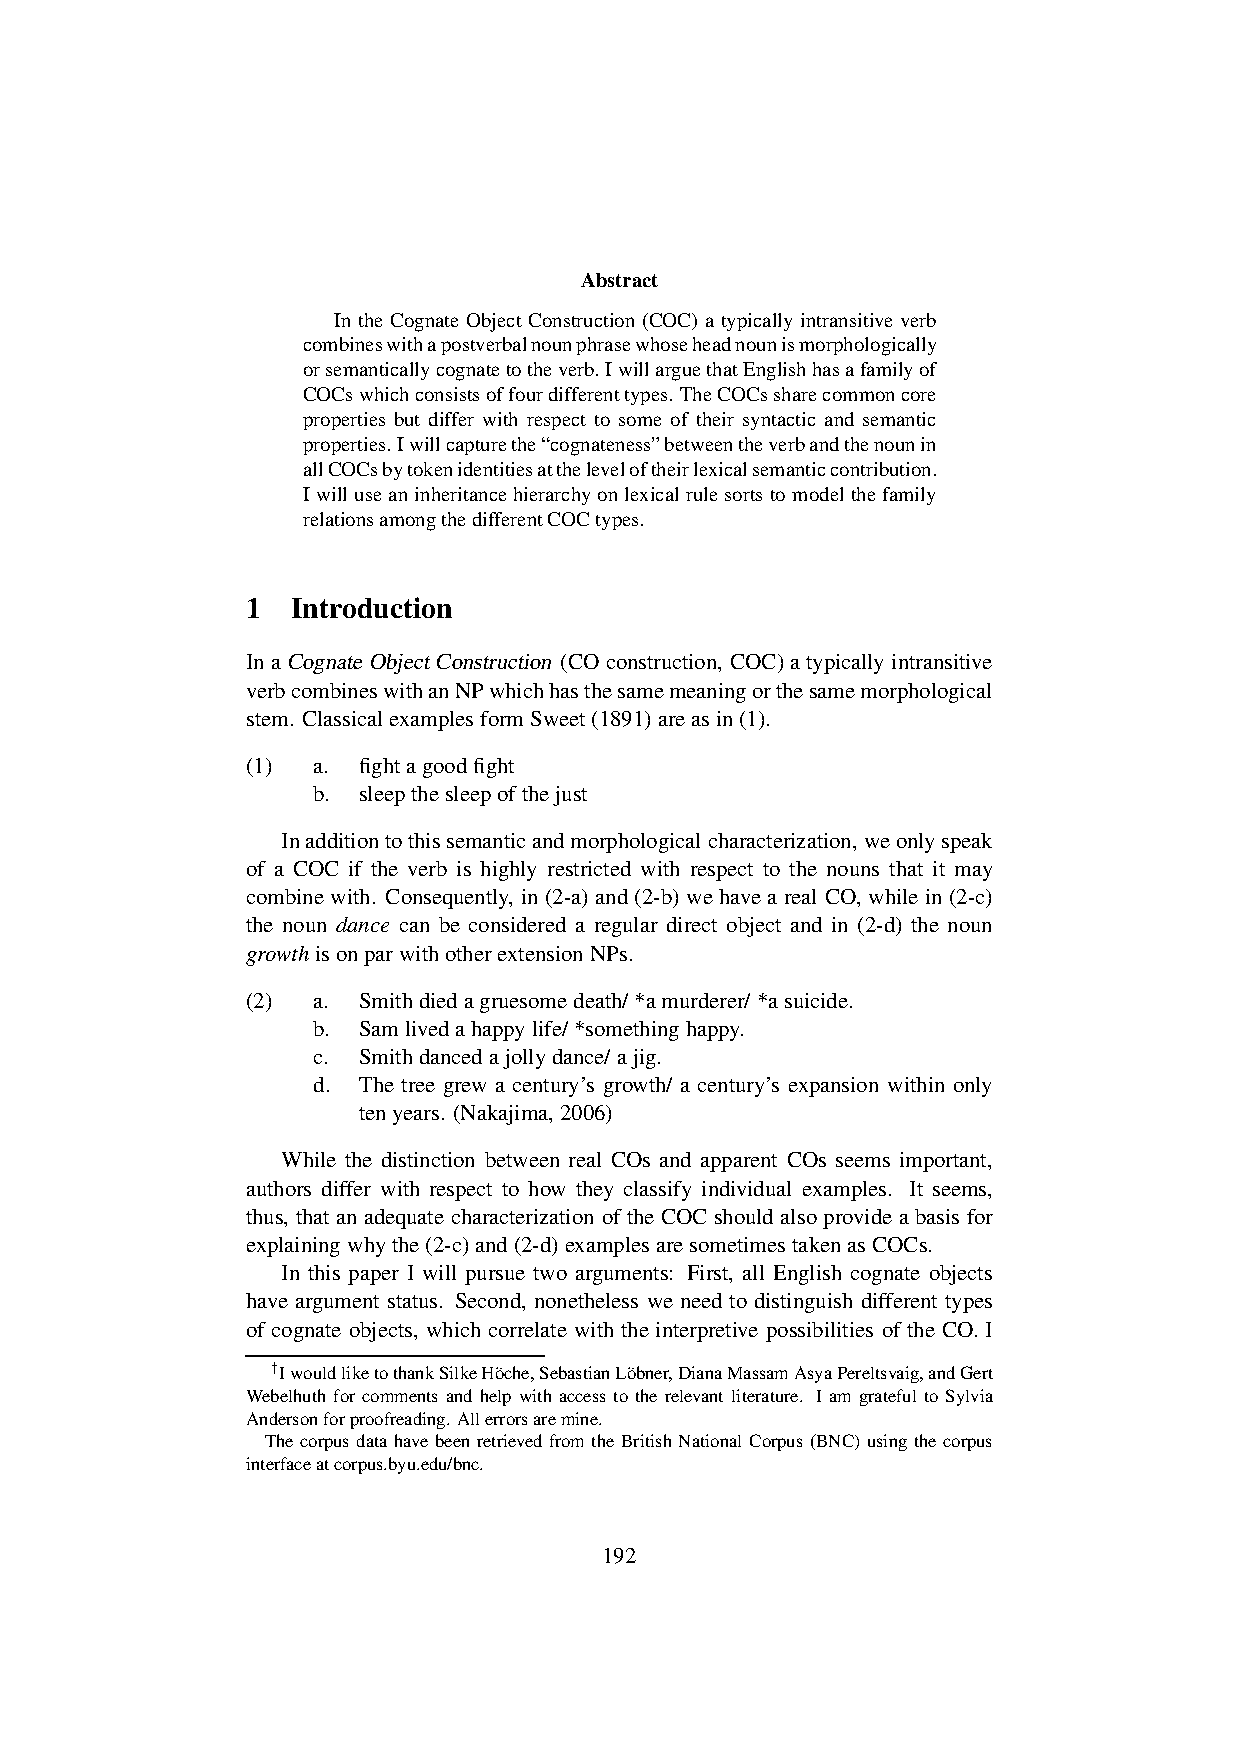
\includepdf[pages=-,pagecommand=\thispagestyle{plain}]{Includes/sailer.pdf}
        \setcounter{page}{212}
        \phantomsection
        \addcontentsline{toc}{section}{Pollet Samvelian, Jesse Tseng: Persian Object Clitics and the Syntax-Morphology Interface}
\thispagestyle{empty}

\begin{center}
  {\huge\bfseries Persian Object Clitics and the Syntax-Morphology Interface\par}

  \bigskip

~\\
\begingroup
\setlength{\leftskip}{0pt plus 1fill}
\setlength{\rightskip}{0pt plus 1fill}
\setlength{\parindent}{0pt}
\setlength{\parfillskip}{0pt}
  \formatauthor{Pollet Samvelian}{\begin{tabular}{@{}c@{}}Université de Paris 3\end{tabular}}
\formatauthor{Jesse Tseng}{\begin{tabular}{@{}c@{}}CNRS\end{tabular}}

\par\endgroup

  \vspace*{8ex}

  Proceedings of the 17th International Conference on\par Head-Driven Phrase Structure Grammar

  \bigskip

  Universit{\'e} Paris Diderot, Paris 7, France

  \medskip

  Stefan Müller (Editor)

  \medskip

  2010

  \medskip

  CSLI Publications

  \medskip

  pages 212--232

  \medskip

  \url{http://csli-publications.stanford.edu/HPSG/2010}
\end{center}
\vfill

\noindent



\vfill
\noindent
% APA Style
Samvelian, Pollet, \& Tseng, Jesse. 2010. Persian Object Clitics and the Syntax-Morphology Interface. In Müller, Stefan (Ed.), \emph{{Proceedings of the 17th International Conference on Head-Driven Phrase Structure Grammar, Universit{\'e} Paris Diderot, Paris 7, France}}, 212--232. Stanford,
CA: CSLI Publications. \hfill\href{http://creativecommons.org/licenses/by/4.0/}{\includegraphics[height=.75em]{Includes/ccby.eps}}

\newpage
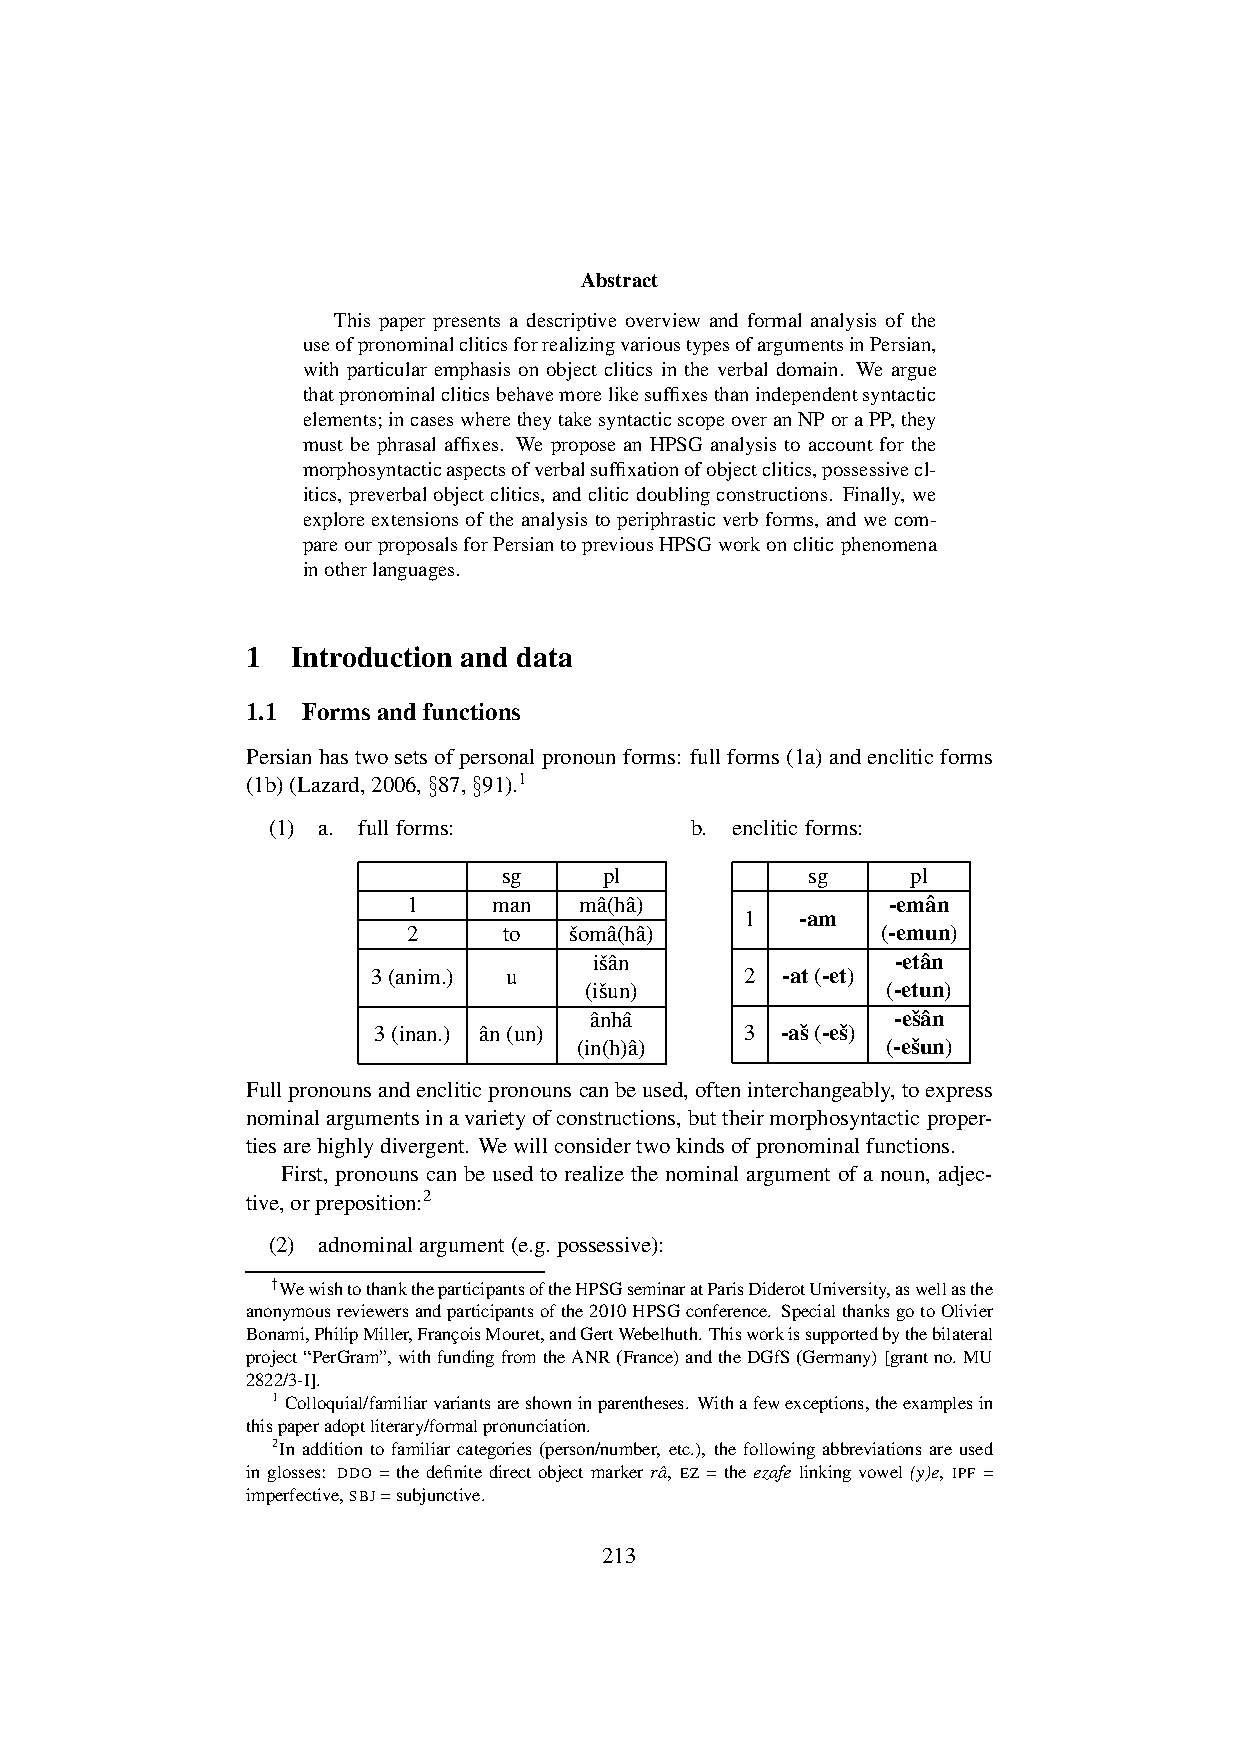
\includepdf[pages=-,pagecommand=\thispagestyle{plain}]{Includes/samvelian-tseng.pdf}
\part{Contributions to the Workshop}
\thispagestyle{empty}
\newpage
        \setcounter{page}{234}
        \phantomsection
        \addcontentsline{toc}{section}{Dunstan Brown, Roger Evans: Inflectional Defaults and Principal Parts: an Empirical Investigation}
\thispagestyle{empty}

\begin{center}
  {\huge\bfseries Inflectional Defaults and Principal Parts: an Empirical Investigation\par}

  \bigskip

~\\
\begingroup
\setlength{\leftskip}{0pt plus 1fill}
\setlength{\rightskip}{0pt plus 1fill}
\setlength{\parindent}{0pt}
\setlength{\parfillskip}{0pt}
  \formatauthor{Dunstan Brown}{\begin{tabular}{@{}c@{}}University of Surrey\end{tabular}}
\formatauthor{Roger Evans}{\begin{tabular}{@{}c@{}}University of Brighton\end{tabular}}

\par\endgroup

  \vspace*{8ex}

  Proceedings of the 17th International Conference on\par Head-Driven Phrase Structure Grammar

  \bigskip

  Universit{\'e} Paris Diderot, Paris 7, France

  \medskip

  Stefan Müller (Editor)

  \medskip

  2010

  \medskip

  CSLI Publications

  \medskip

  pages 234--254

  \medskip

  \url{http://csli-publications.stanford.edu/HPSG/2010}
\end{center}
\vfill

\noindent



\vfill
\noindent
% APA Style
Brown, Dunstan, \& Evans, Roger. 2010. Inflectional Defaults and Principal Parts: an Empirical Investigation. In Müller, Stefan (Ed.), \emph{{Proceedings of the 17th International Conference on Head-Driven Phrase Structure Grammar, Universit{\'e} Paris Diderot, Paris 7, France}}, 234--254. Stanford,
CA: CSLI Publications. \hfill\href{http://creativecommons.org/licenses/by/4.0/}{\includegraphics[height=.75em]{Includes/ccby.eps}}

\newpage
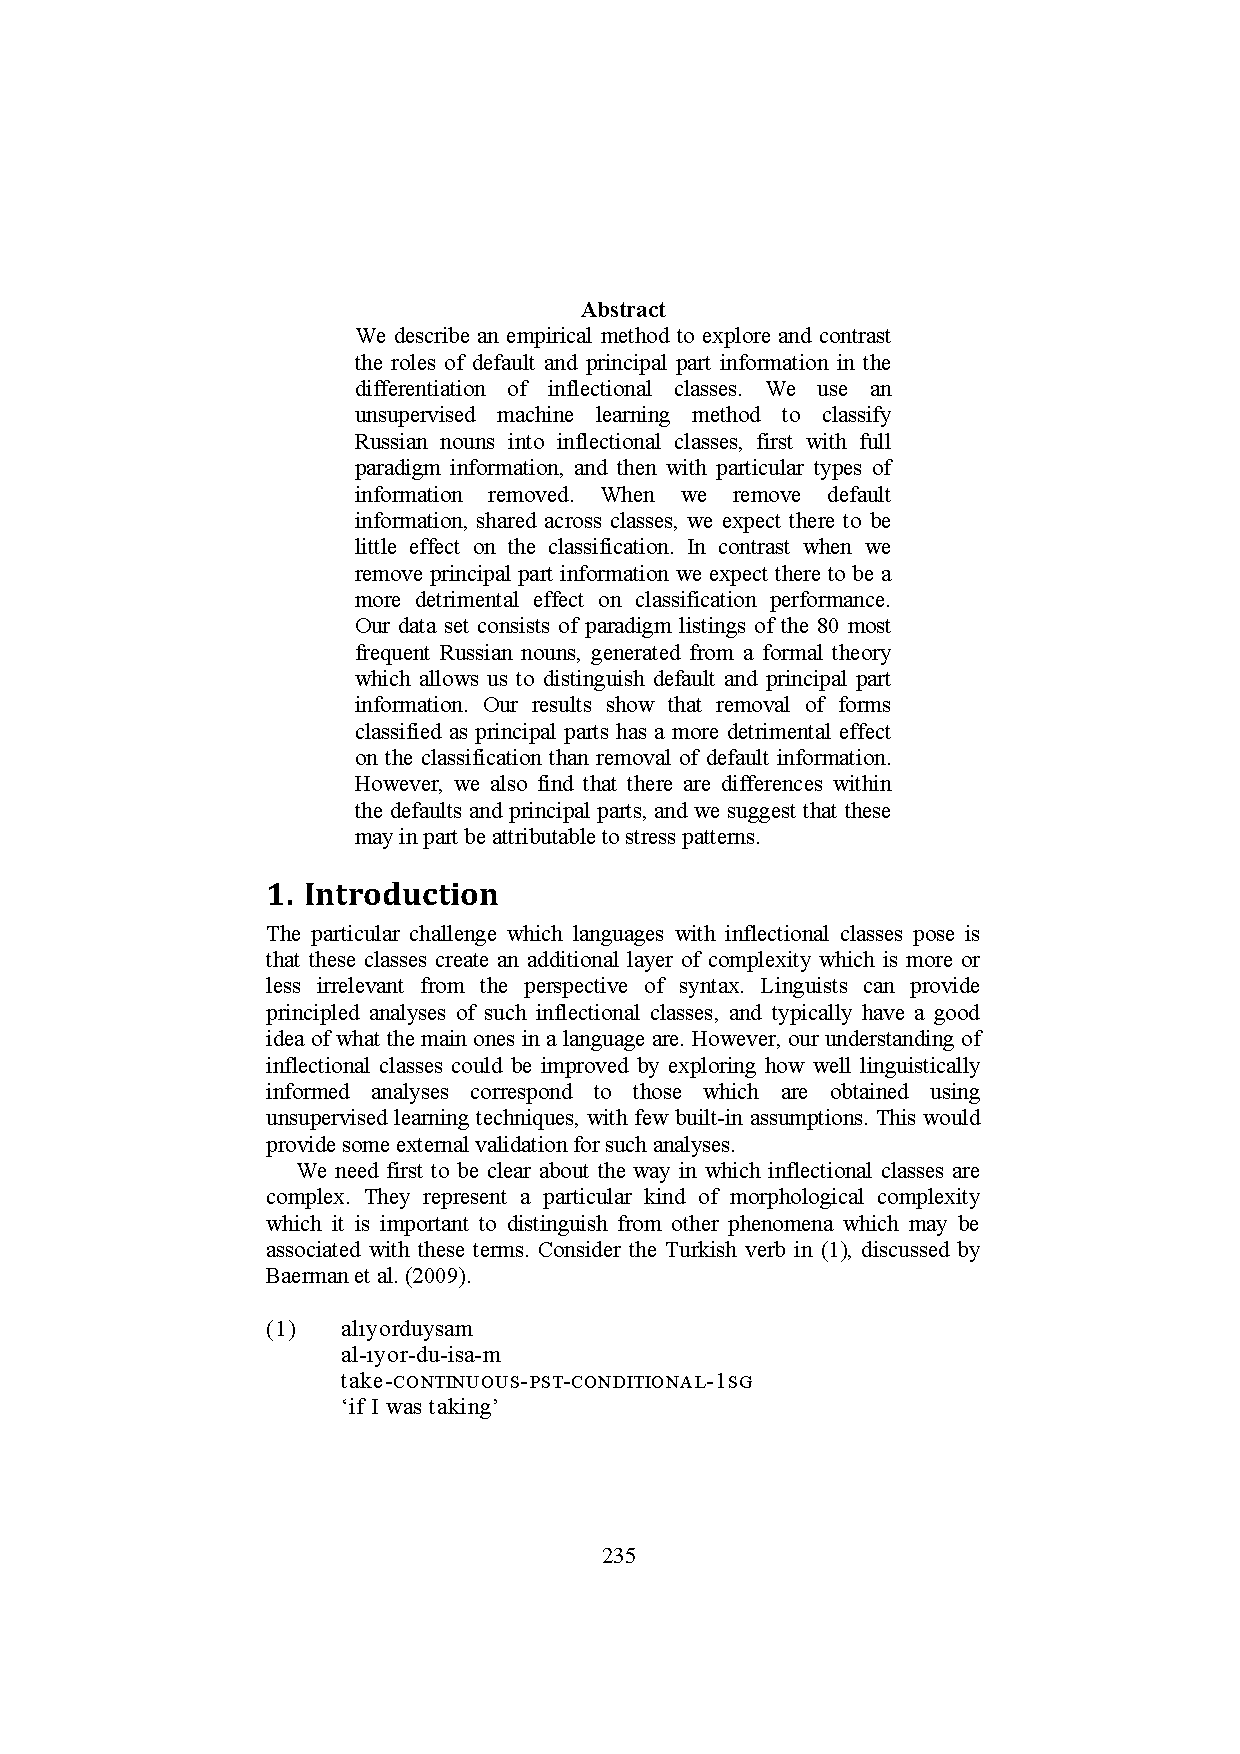
\includepdf[pages=-,pagecommand=\thispagestyle{plain}]{Includes/brown-evans.pdf}
        \setcounter{page}{255}
        \phantomsection
        \addcontentsline{toc}{section}{Greville G. Corbett: Classic Problems at the Syntax-Morphology Interface:\\ Whose are They?}
\thispagestyle{empty}

\begin{center}
  {\huge\bfseries Classic Problems at the Syntax-Morphology Interface:\par Whose are They?\par}

  \bigskip

~\\
\begingroup
\setlength{\leftskip}{0pt plus 1fill}
\setlength{\rightskip}{0pt plus 1fill}
\setlength{\parindent}{0pt}
\setlength{\parfillskip}{0pt}
  \formatauthor{Greville G. Corbett}{\begin{tabular}{@{}c@{}}University of Surrey\end{tabular}}

\par\endgroup

  \vspace*{8ex}

  Proceedings of the 17th International Conference on\par Head-Driven Phrase Structure Grammar

  \bigskip

  Universit{\'e} Paris Diderot, Paris 7, France

  \medskip

  Stefan Müller (Editor)

  \medskip

  2010

  \medskip

  CSLI Publications

  \medskip

  pages 255--268

  \medskip

  \url{http://csli-publications.stanford.edu/HPSG/2010}
\end{center}
\vfill

\noindent



\vfill
\noindent
% APA Style
Corbett, Greville G. 2010. Classic Problems at the Syntax-Morphology Interface:  Whose are They? In Müller, Stefan (Ed.), \emph{{Proceedings of the 17th International Conference on Head-Driven Phrase Structure Grammar, Universit{\'e} Paris Diderot, Paris 7, France}}, 255--268. Stanford,
CA: CSLI Publications. \hfill\href{http://creativecommons.org/licenses/by/4.0/}{\includegraphics[height=.75em]{Includes/ccby.eps}}

\newpage
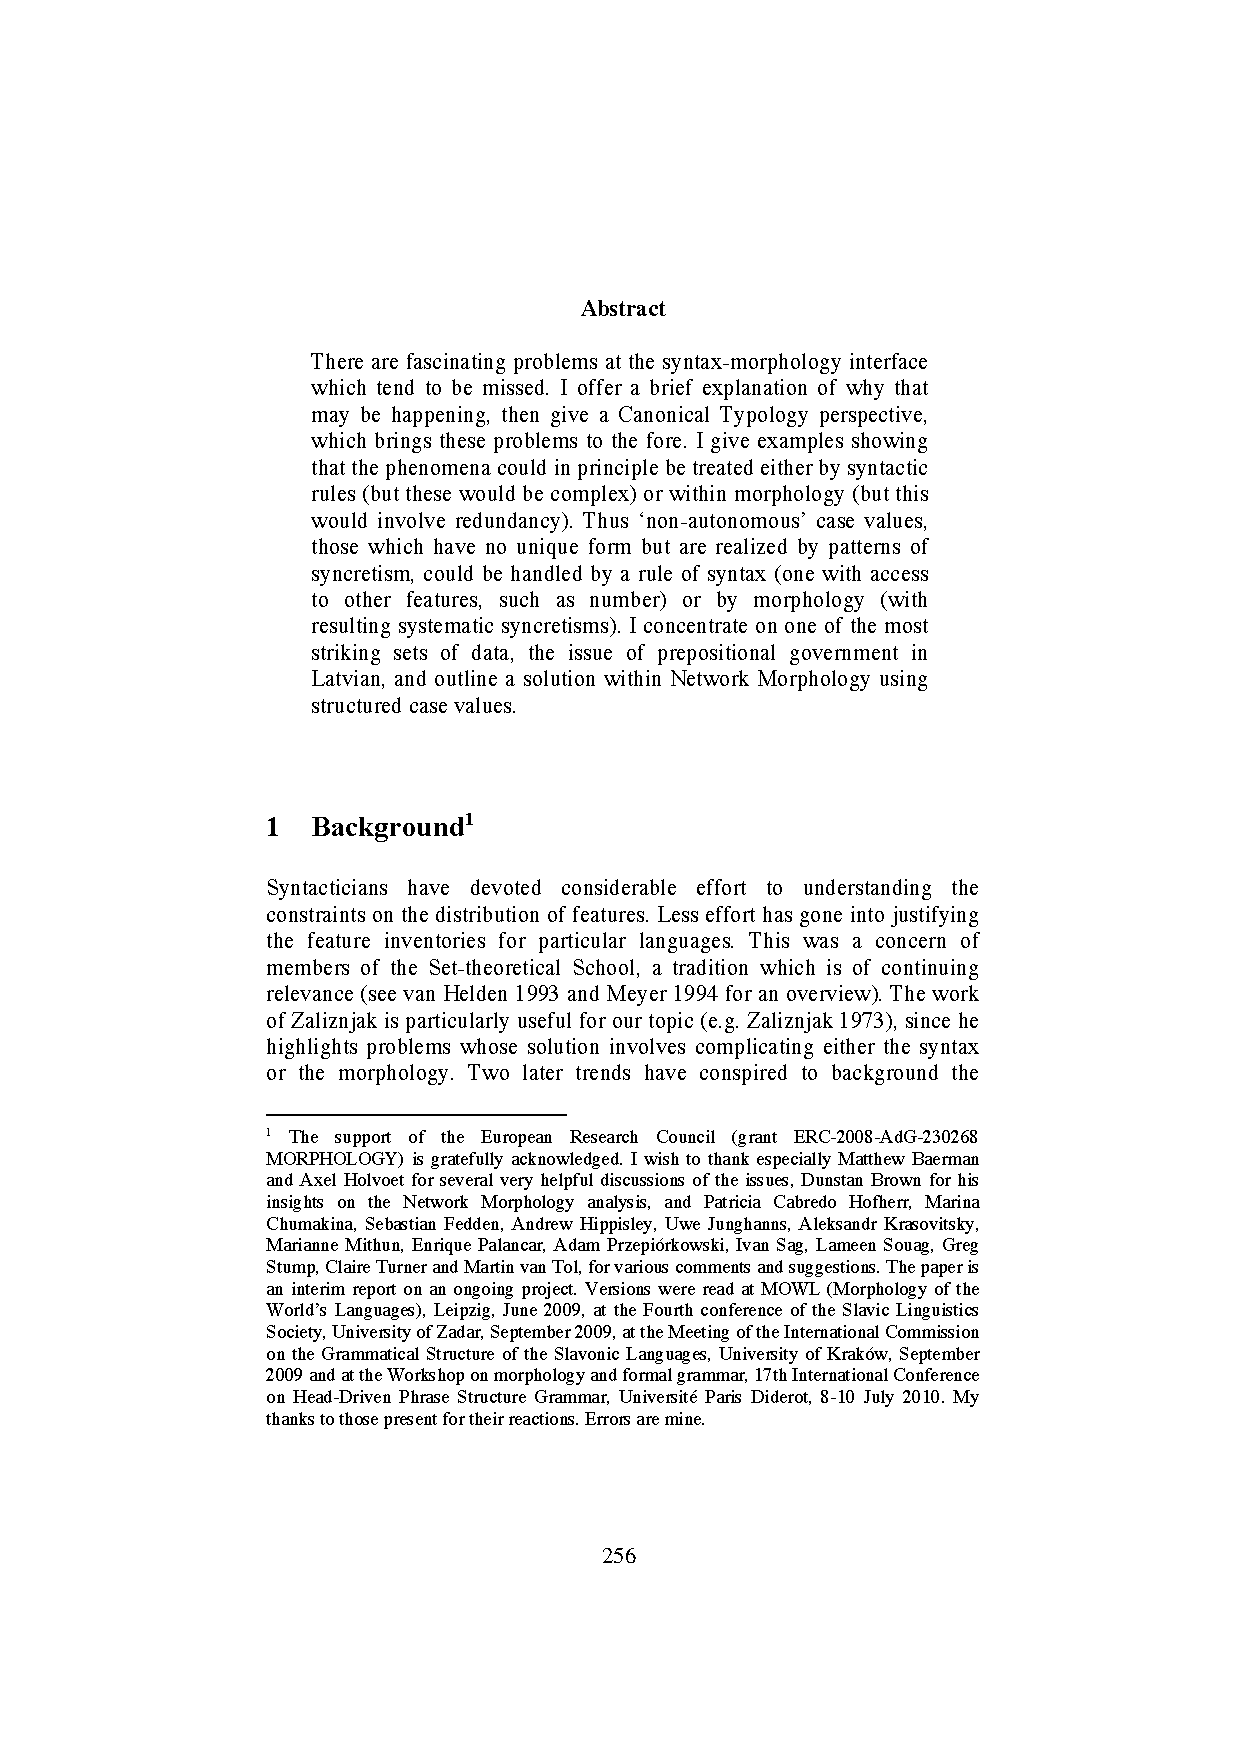
\includepdf[pages=-,pagecommand=\thispagestyle{plain}]{Includes/corbett.pdf}
        \setcounter{page}{269}
        \phantomsection
        \addcontentsline{toc}{section}{Berthold Crysmann: Discontinuous Negation in Hausa}
\thispagestyle{empty}

\begin{center}
  {\huge\bfseries Discontinuous Negation in Hausa\par}

  \bigskip

~\\
\begingroup
\setlength{\leftskip}{0pt plus 1fill}
\setlength{\rightskip}{0pt plus 1fill}
\setlength{\parindent}{0pt}
\setlength{\parfillskip}{0pt}
  \formatauthor{Berthold Crysmann}{\begin{tabular}{@{}c@{}}Universität Bonn and Universität des Saarlandes\end{tabular}}

\par\endgroup

  \vspace*{8ex}

  Proceedings of the 17th International Conference on\par Head-Driven Phrase Structure Grammar

  \bigskip

  Universit{\'e} Paris Diderot, Paris 7, France

  \medskip

  Stefan Müller (Editor)

  \medskip

  2010

  \medskip

  CSLI Publications

  \medskip

  pages 269--287

  \medskip

  \url{http://csli-publications.stanford.edu/HPSG/2010}
\end{center}
\vfill

\noindent



\vfill
\noindent
% APA Style
Crysmann, Berthold. 2010. Discontinuous Negation in Hausa. In Müller, Stefan (Ed.), \emph{{Proceedings of the 17th International Conference on Head-Driven Phrase Structure Grammar, Universit{\'e} Paris Diderot, Paris 7, France}}, 269--287. Stanford,
CA: CSLI Publications. \hfill\href{http://creativecommons.org/licenses/by/4.0/}{\includegraphics[height=.75em]{Includes/ccby.eps}}

\newpage
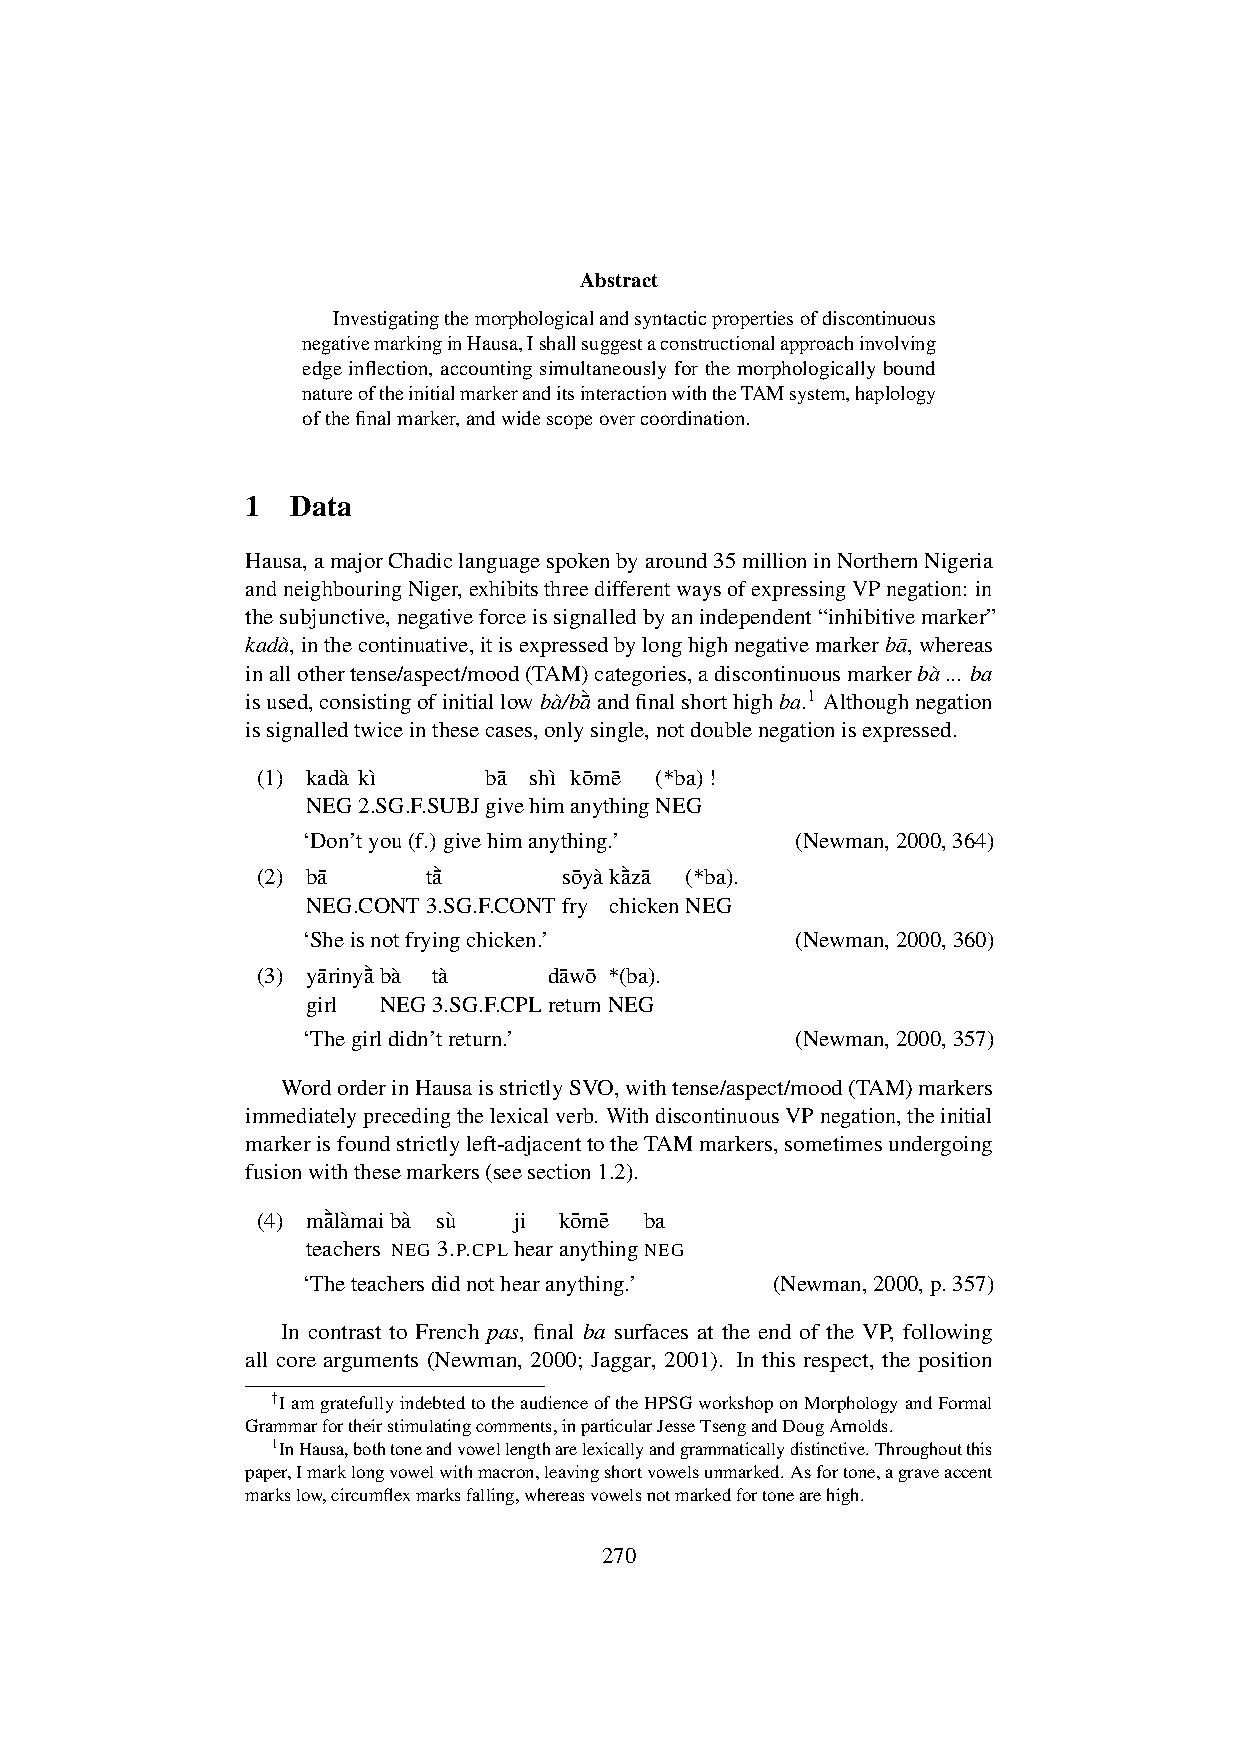
\includepdf[pages=-,pagecommand=\thispagestyle{plain}]{Includes/crysmann.pdf}
        \setcounter{page}{288}
        \phantomsection
        \addcontentsline{toc}{section}{Jean-L{\'e}o L{\'e}onard, Alain Kihm: Verb Inflection in Chiquihuitlán Mazatec: a Fragment and a PFM Approach}
\thispagestyle{empty}

\begin{center}
  {\huge\bfseries Verb Inflection in Chiquihuitlán Mazatec: a Fragment and a PFM Approach\par}

  \bigskip

~\\
\begingroup
\setlength{\leftskip}{0pt plus 1fill}
\setlength{\rightskip}{0pt plus 1fill}
\setlength{\parindent}{0pt}
\setlength{\parfillskip}{0pt}
  \formatauthor{Jean-Léo Léonard}{\begin{tabular}{@{}c@{}}Paris 3, IUF\end{tabular}}
\formatauthor{Alain Kihm}{\begin{tabular}{@{}c@{}}CNRS, Paris 7\end{tabular}}

\par\endgroup

  \vspace*{8ex}

  Proceedings of the 17th International Conference on\par Head-Driven Phrase Structure Grammar

  \bigskip

  Universit{\'e} Paris Diderot, Paris 7, France

  \medskip

  Stefan Müller (Editor)

  \medskip

  2010

  \medskip

  CSLI Publications

  \medskip

  pages 288--306

  \medskip

  \url{http://csli-publications.stanford.edu/HPSG/2010}
\end{center}
\vfill

\noindent



\vfill
\noindent
% APA Style
Léonard, Jean-Léo, \& Kihm, Alain. 2010. Verb Inflection in Chiquihuitlán Mazatec: a Fragment and a PFM Approach. In Müller, Stefan (Ed.), \emph{{Proceedings of the 17th International Conference on Head-Driven Phrase Structure Grammar, Universit{\'e} Paris Diderot, Paris 7, France}}, 288--306. Stanford,
CA: CSLI Publications. \hfill\href{http://creativecommons.org/licenses/by/4.0/}{\includegraphics[height=.75em]{Includes/ccby.eps}}

\newpage
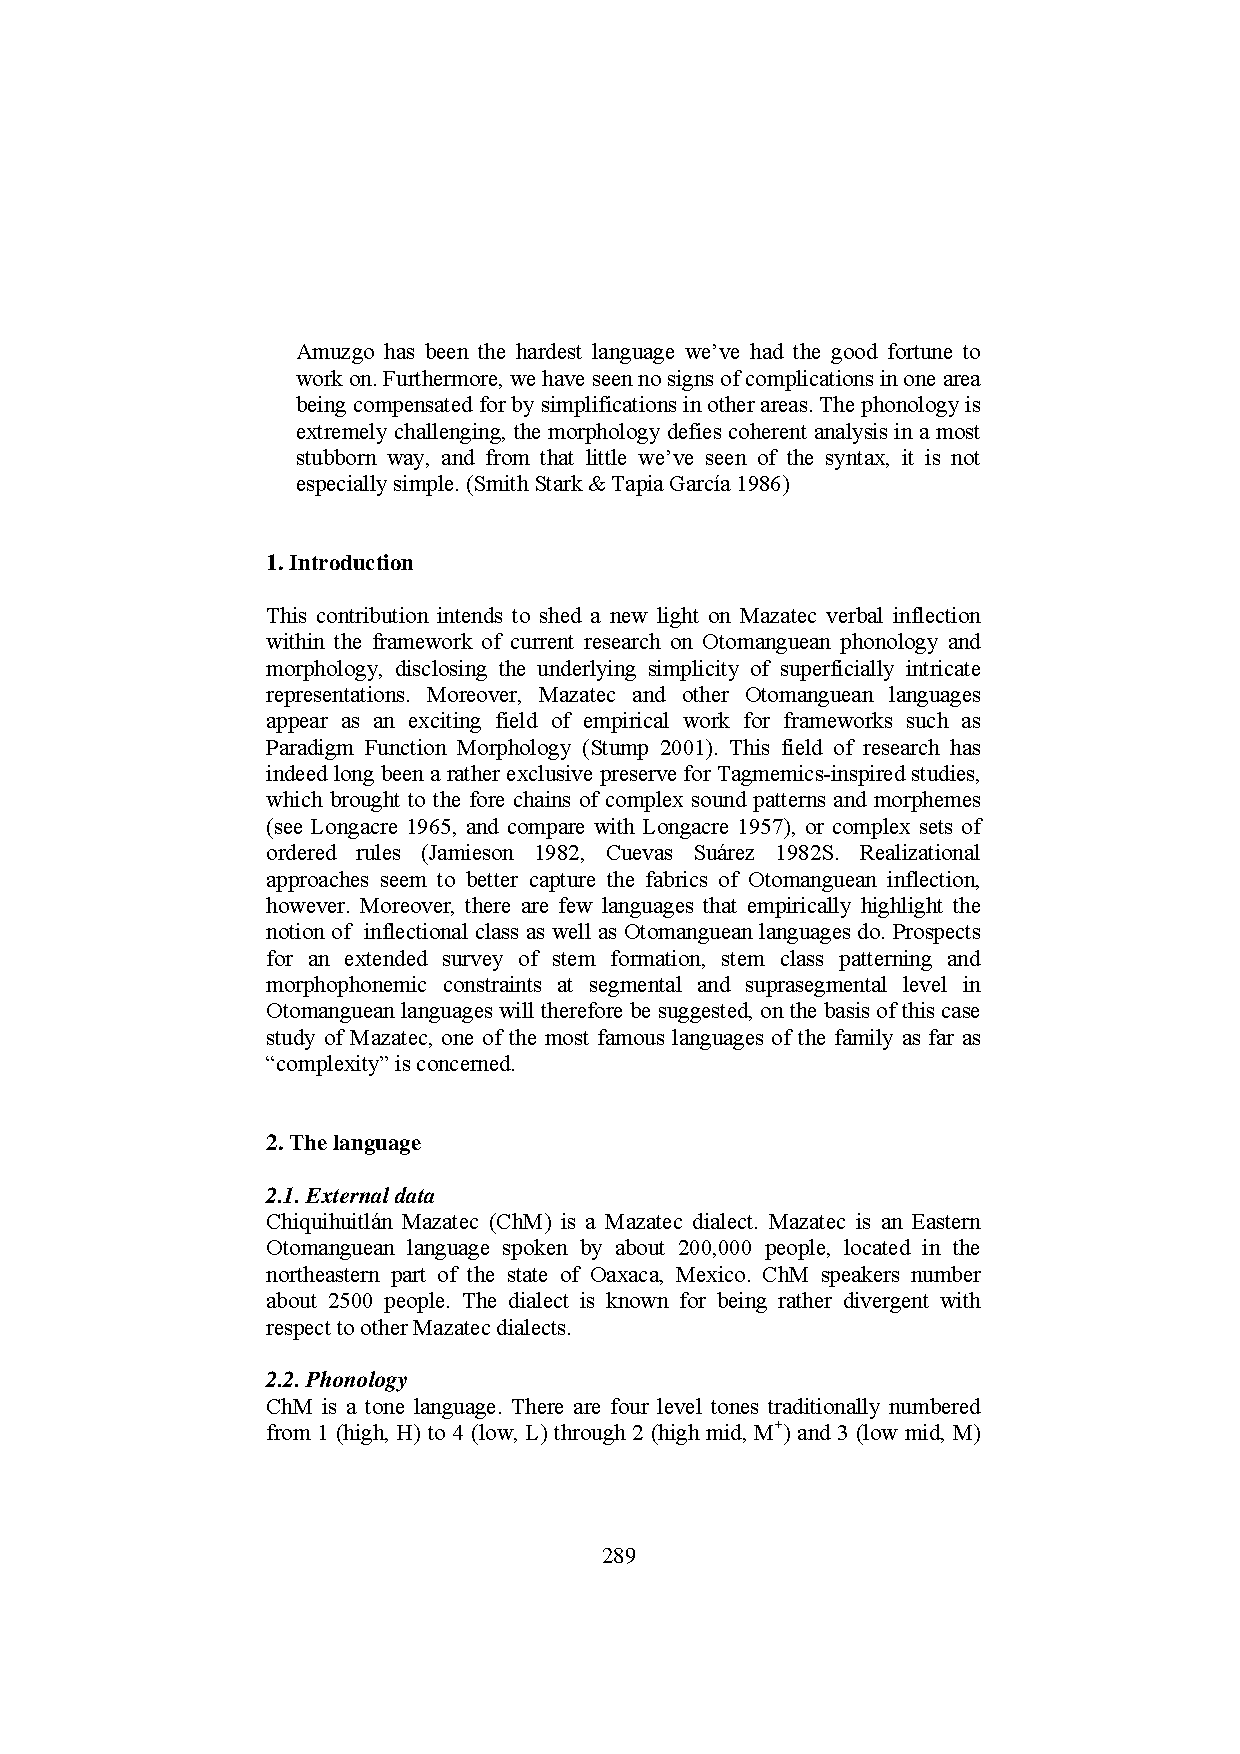
\includepdf[pages=-,pagecommand=\thispagestyle{plain}]{Includes/leonard-kihm.pdf}
        \setcounter{page}{307}
        \phantomsection
        \addcontentsline{toc}{section}{Smriti Singh, Vaijayanthi M Sarma: Hindi Noun Inflection and Distributed Morphology}
\thispagestyle{empty}

\begin{center}
  {\huge\bfseries Hindi Noun Inflection and Distributed Morphology\par}

  \bigskip

~\\
\begingroup
\setlength{\leftskip}{0pt plus 1fill}
\setlength{\rightskip}{0pt plus 1fill}
\setlength{\parindent}{0pt}
\setlength{\parfillskip}{0pt}
  \formatauthor{Smriti Singh}{\begin{tabular}{@{}c@{}}Indian Institute of Technology Bombay\end{tabular}}
\formatauthor{Vaijayanthi M Sarma}{\begin{tabular}{@{}c@{}}Indian Institute of Technology Bombay\end{tabular}}

\par\endgroup

  \vspace*{8ex}

  Proceedings of the 17th International Conference on\par Head-Driven Phrase Structure Grammar

  \bigskip

  Universit{\'e} Paris Diderot, Paris 7, France

  \medskip

  Stefan Müller (Editor)

  \medskip

  2010

  \medskip

  CSLI Publications

  \medskip

  pages 307--321

  \medskip

  \url{http://csli-publications.stanford.edu/HPSG/2010}
\end{center}
\vfill

\noindent



\vfill
\noindent
% APA Style
Singh, Smriti, \& Sarma, Vaijayanthi M. 2010. Hindi Noun Inflection and Distributed Morphology. In Müller, Stefan (Ed.), \emph{{Proceedings of the 17th International Conference on Head-Driven Phrase Structure Grammar, Universit{\'e} Paris Diderot, Paris 7, France}}, 307--321. Stanford,
CA: CSLI Publications. \hfill\href{http://creativecommons.org/licenses/by/4.0/}{\includegraphics[height=.75em]{Includes/ccby.eps}}

\newpage
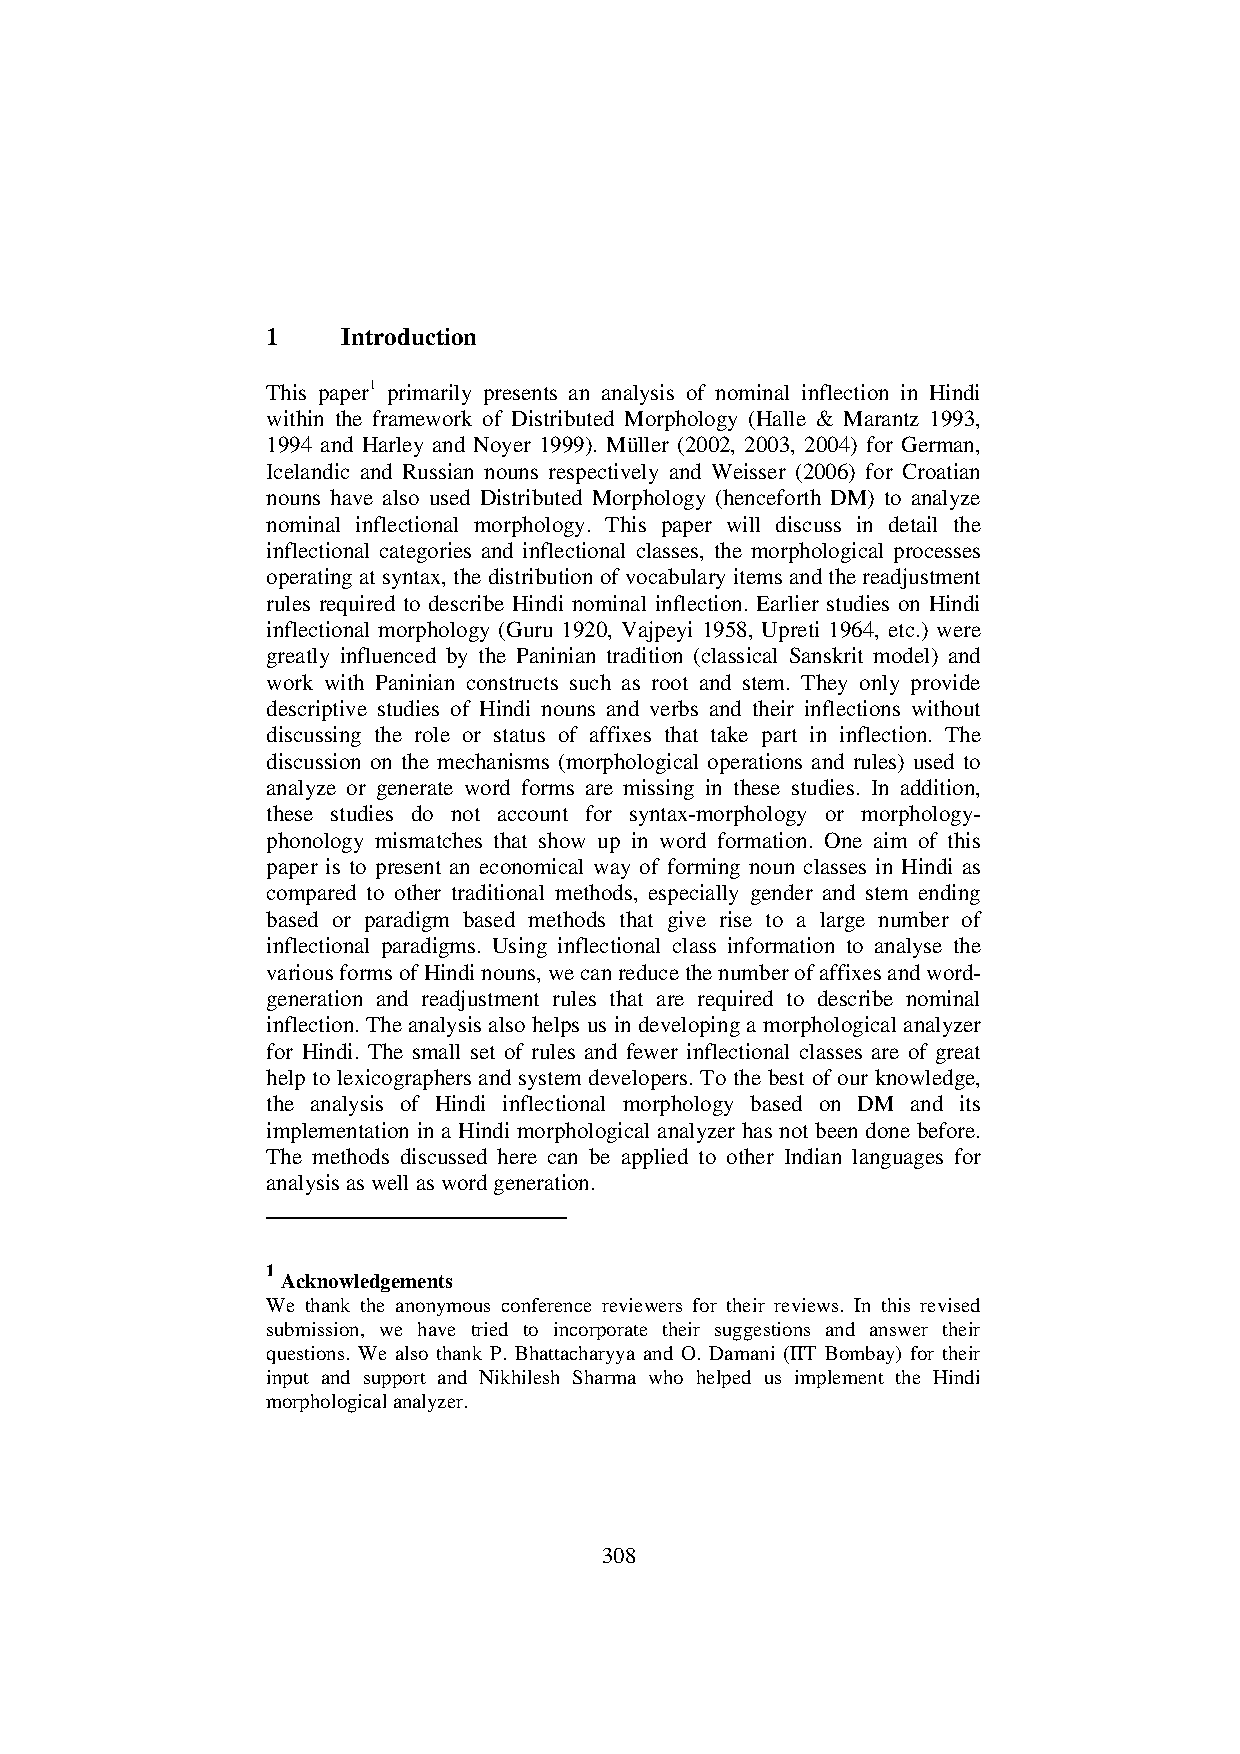
\includepdf[pages=-,pagecommand=\thispagestyle{plain}]{Includes/singh-sarma.pdf}
        \setcounter{page}{322}
        \phantomsection
        \addcontentsline{toc}{section}{Andrew Spencer: Lexical Relatedness and the Lexical Entry -- a Formal Unification}
\thispagestyle{empty}

\begin{center}
  {\huge\bfseries Lexical Relatedness and the Lexical Entry -- a Formal Unification\par}

  \bigskip

~\\
\begingroup
\setlength{\leftskip}{0pt plus 1fill}
\setlength{\rightskip}{0pt plus 1fill}
\setlength{\parindent}{0pt}
\setlength{\parfillskip}{0pt}
  \formatauthor{Andrew Spencer}{\begin{tabular}{@{}c@{}}University of Essex\end{tabular}}

\par\endgroup

  \vspace*{8ex}

  Proceedings of the 17th International Conference on\par Head-Driven Phrase Structure Grammar

  \bigskip

  Universit{\'e} Paris Diderot, Paris 7, France

  \medskip

  Stefan Müller (Editor)

  \medskip

  2010

  \medskip

  CSLI Publications

  \medskip

  pages 322--340

  \medskip

  \url{http://csli-publications.stanford.edu/HPSG/2010}
\end{center}
\vfill

\noindent



\vfill
\noindent
% APA Style
Spencer, Andrew. 2010. Lexical Relatedness and the Lexical Entry -- a Formal Unification. In Müller, Stefan (Ed.), \emph{{Proceedings of the 17th International Conference on Head-Driven Phrase Structure Grammar, Universit{\'e} Paris Diderot, Paris 7, France}}, 322--340. Stanford,
CA: CSLI Publications. \hfill\href{http://creativecommons.org/licenses/by/4.0/}{\includegraphics[height=.75em]{Includes/ccby.eps}}

\newpage
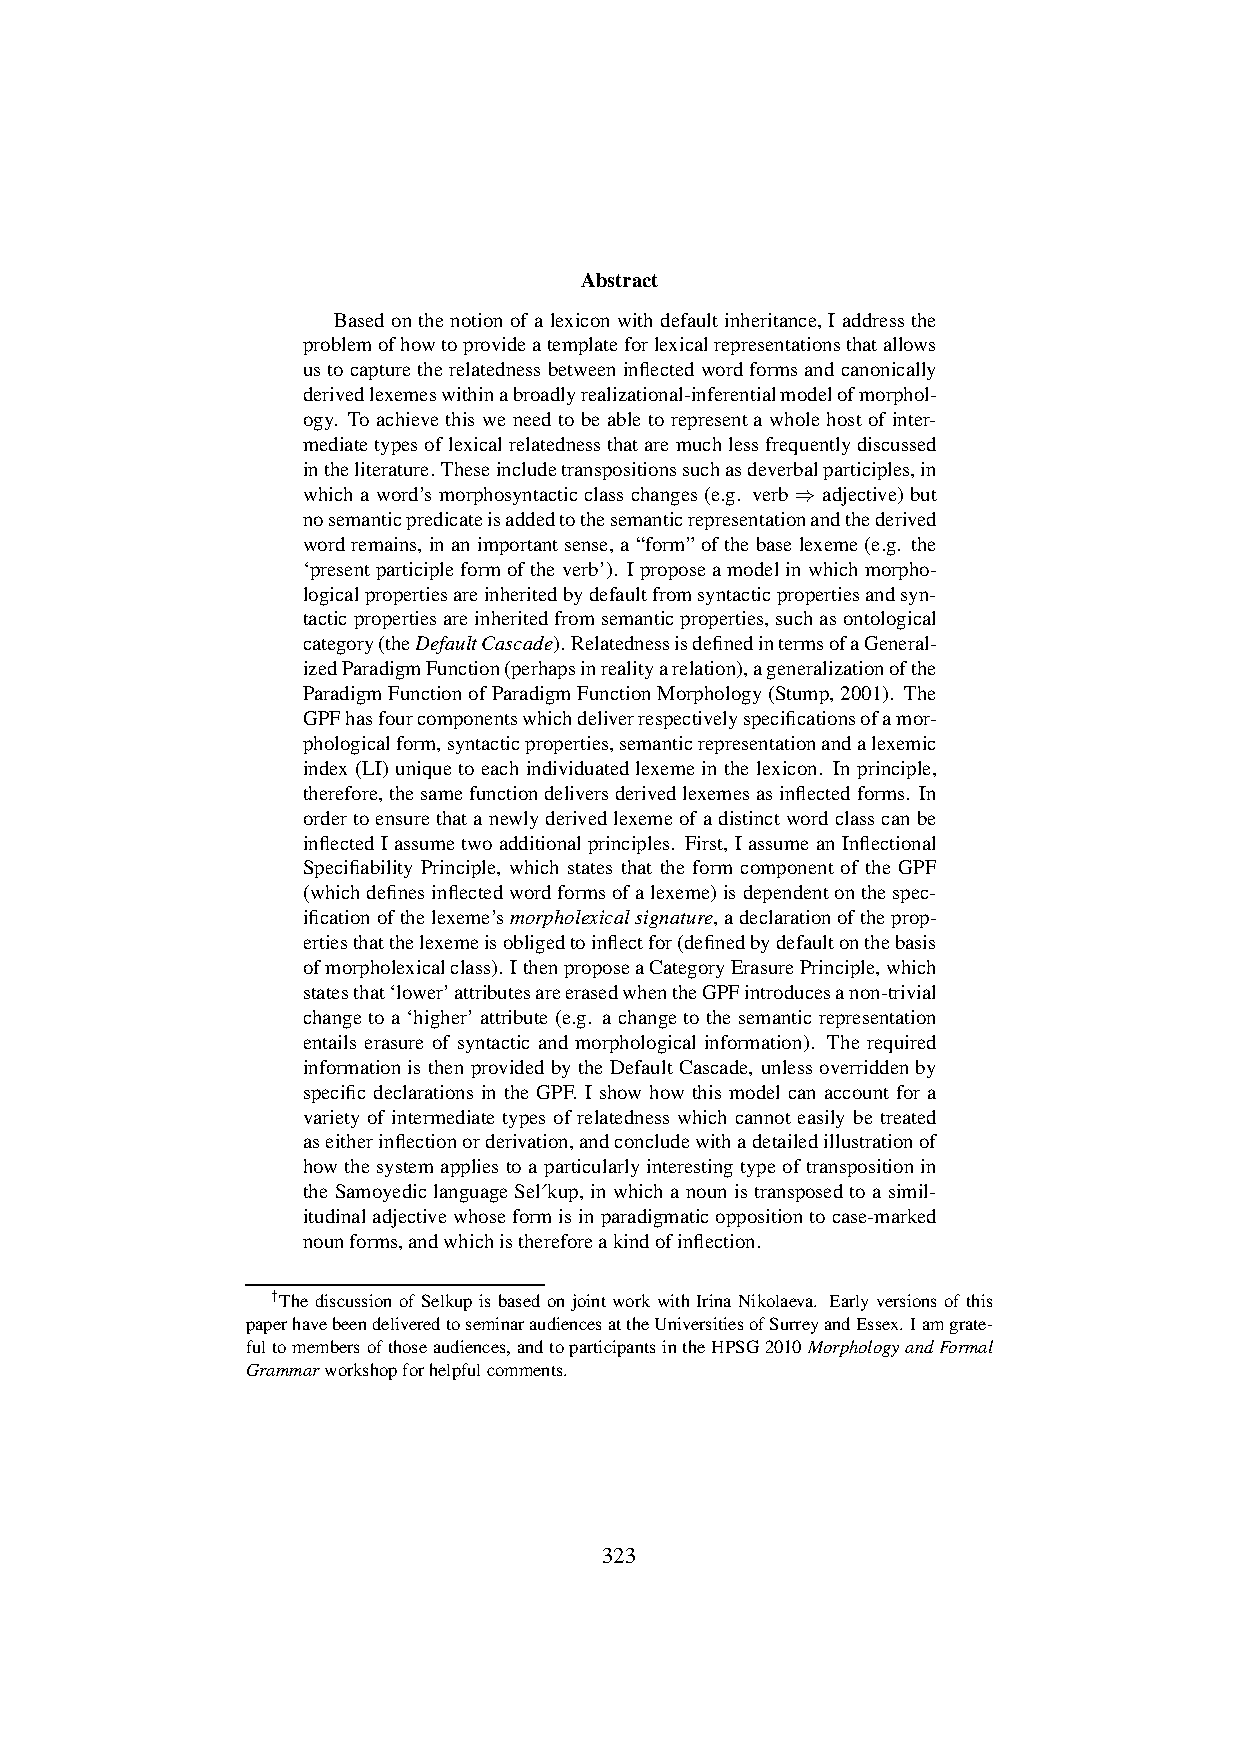
\includepdf[pages=-,pagecommand=\thispagestyle{plain}]{Includes/spencer.pdf}
        \setcounter{page}{341}
        \phantomsection
        \addcontentsline{toc}{section}{Delphine Tribout: How Many Conversions from Verb to Noun Are There in French?}
\thispagestyle{empty}

\begin{center}
  {\huge\bfseries How Many Conversions from Verb to Noun Are There in French?\par}

  \bigskip

~\\
\begingroup
\setlength{\leftskip}{0pt plus 1fill}
\setlength{\rightskip}{0pt plus 1fill}
\setlength{\parindent}{0pt}
\setlength{\parfillskip}{0pt}
  \formatauthor{Delphine Tribout}{\begin{tabular}{@{}c@{}}LLF and Université Paris Diderot-Paris 7\end{tabular}}

\par\endgroup

  \vspace*{8ex}

  Proceedings of the 17th International Conference on\par Head-Driven Phrase Structure Grammar

  \bigskip

  Universit{\'e} Paris Diderot, Paris 7, France

  \medskip

  Stefan Müller (Editor)

  \medskip

  2010

  \medskip

  CSLI Publications

  \medskip

  pages 341--357

  \medskip

  \url{http://csli-publications.stanford.edu/HPSG/2010}
\end{center}
\vfill

\noindent



\vfill
\noindent
% APA Style
Tribout, Delphine. 2010. How Many Conversions from Verb to Noun Are There in French? In Müller, Stefan (Ed.), \emph{{Proceedings of the 17th International Conference on Head-Driven Phrase Structure Grammar, Universit{\'e} Paris Diderot, Paris 7, France}}, 341--357. Stanford,
CA: CSLI Publications. \hfill\href{http://creativecommons.org/licenses/by/4.0/}{\includegraphics[height=.75em]{Includes/ccby.eps}}

\newpage
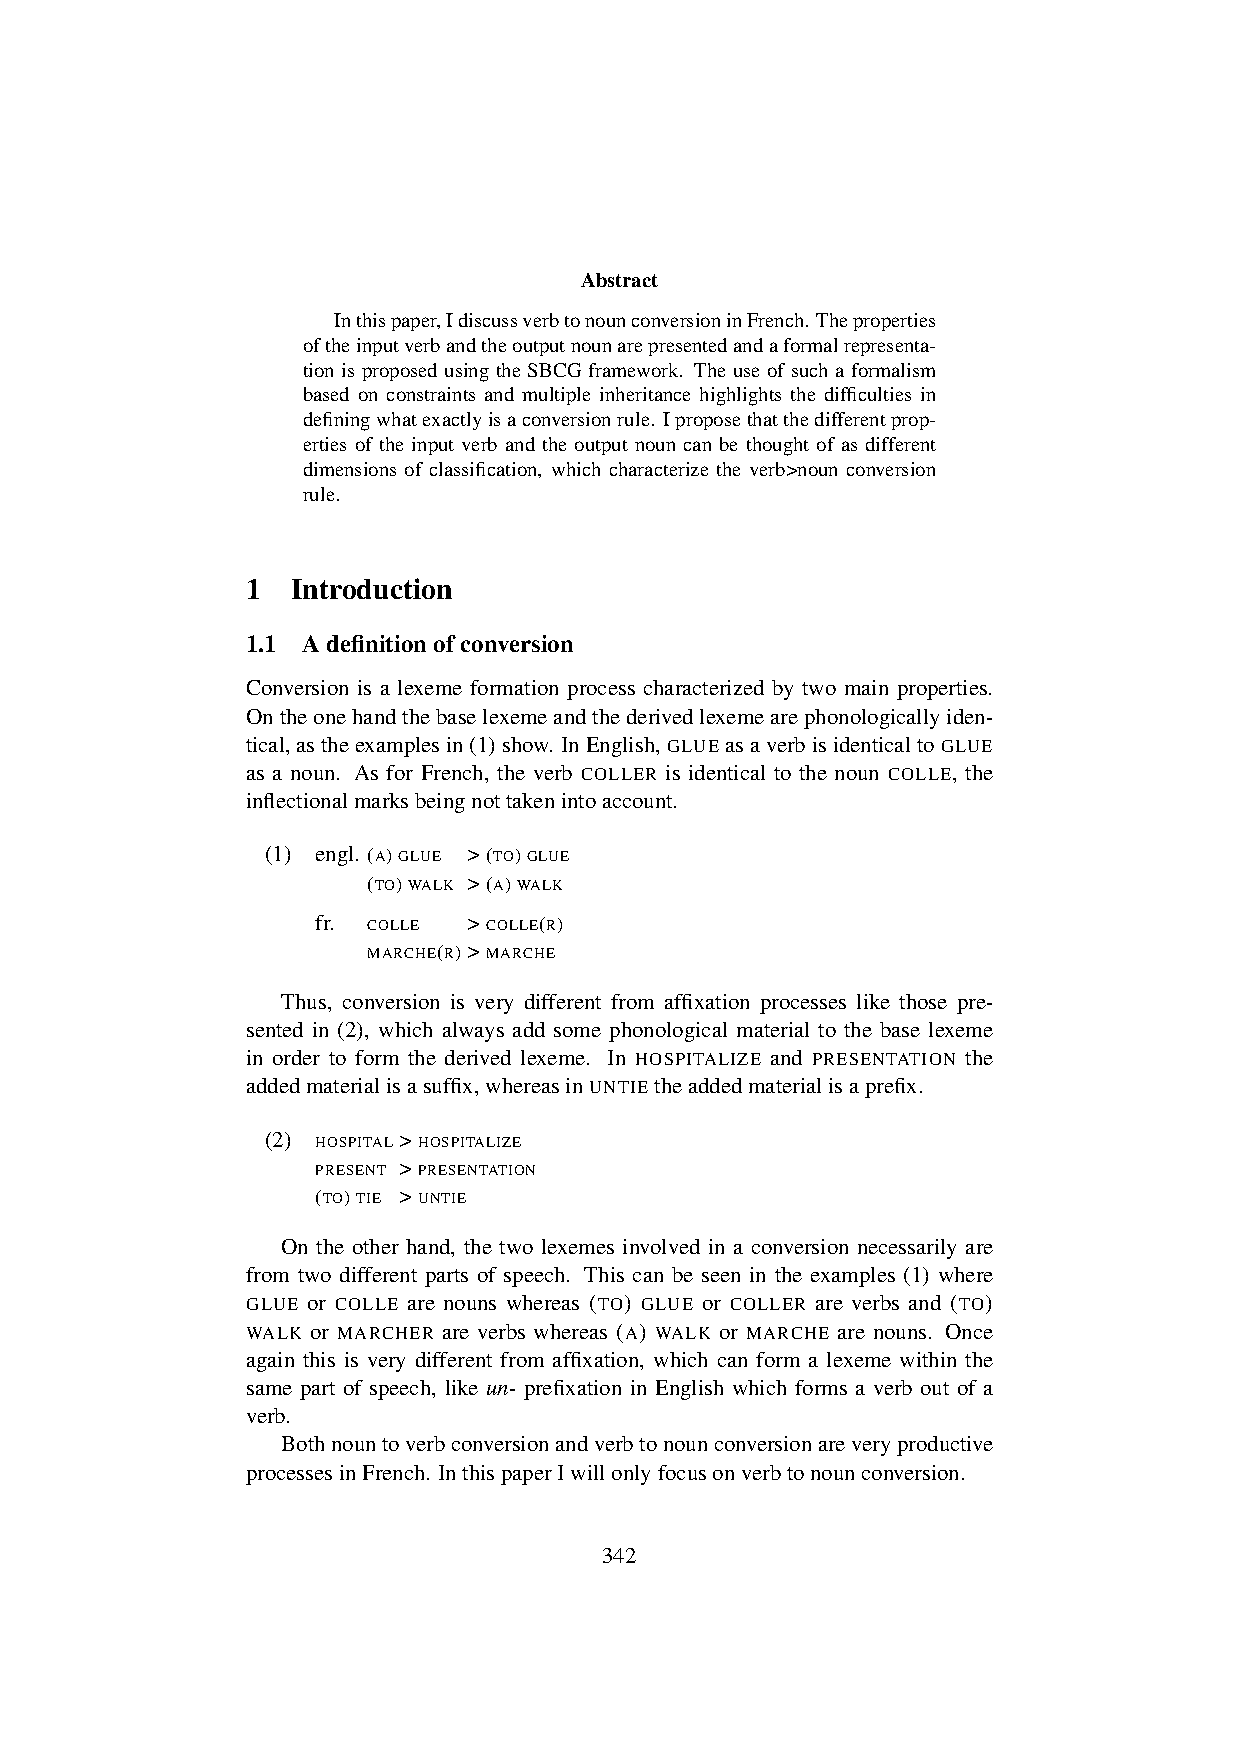
\includepdf[pages=-,pagecommand=\thispagestyle{plain}]{Includes/tribout.pdf}
\end{document}
